\documentclass[conference]{IEEEtran}


%\usepackage{geometry}
\usepackage{amsmath}
\usepackage{amssymb}
\usepackage{amsthm}
\usepackage{times}
\usepackage{helvet}
\usepackage{courier}
\usepackage{graphicx}
\usepackage{subfigure}
\usepackage{mdwmath}
\usepackage{mdwtab}
\usepackage{amssymb}
\usepackage{booktabs}
\usepackage{algorithm}
\usepackage{pifont}
\usepackage{algpseudocode}
\usepackage{balance}
\usepackage{bm}
\usepackage{ulem}
\usepackage{array}
\usepackage{balance}
\usepackage{multirow}
\usepackage{multicol}
\usepackage{threeparttable}
\frenchspacing
\usepackage[marginal]{footmisc}
\usepackage{extarrows}
\usepackage{natbib}

%add the command initial
\algnewcommand\algorithmicInitial{\textbf{Initialize:}}
\algnewcommand\Initial{\item[\algorithmicInitial]}
\algnewcommand\algorithmicIterate{\textbf{Iterate:}}
\algnewcommand\Iterate{\item[\algorithmicIterate]}



\ifCLASSINFOpdf

\else

\fi



% correct bad hyphenation here
\hyphenation{op-tical net-works semi-conduc-tor}


\begin{document}
%
% paper title
% Titles are generally capitalized except for words such as a, an, and, as,
% at, but, by, for, in, nor, of, on, or, the, to and up, which are usually
% not capitalized unless they are the first or last word of the title.
% Linebreaks \\ can be used within to get better formatting as desired.
% Do not put math or special symbols in the title.
%\title{Bare Demo of IEEEtran.cls\\ for IEEE Conferences}
\title{Speed Maintained SVRG}

% author names and affiliations
% use a multiple column layout for up to three different
% affiliations
\author{\IEEEauthorblockN{Erxue Min}
\IEEEauthorblockA{National University of \\Defense Technology\\
Email: mex338@qq.com
}
%Georgia Institute of Technology\\
%Atlanta, Georgia 30332--0250\\
%Email: http://www.michaelshell.org/contact.html}
\and
\IEEEauthorblockN{Yawei Zhao}
\IEEEauthorblockA{National University of \\Defense Technology\\
Email: zhaoyawei09@163.com}
%Springfield, USA\\
%Email: homer@thesimpsons.com}
\and
\IEEEauthorblockN{Jun Long}
\IEEEauthorblockA{National University of \\Defense Technology\\
Email: 14241368@qq.com}}
%San Francisco, California 96678--2391\\
%Telephone: (800) 555--1212\\
%Fax: (888) 555--1212}}

% conference papers do not typically use \thanks and this command
% is locked out in conference mode. If really needed, such as for
% the acknowledgment of grants, issue a \IEEEoverridecommandlockouts
% after \documentclass

% for over three affiliations, or if they all won't fit within the width
% of the page, use this alternative format:
% 
%\author{\IEEEauthorblockN{Michael Shell\IEEEauthorrefmark{1},
%Homer Simpson\IEEEauthorrefmark{2},
%James Kirk\IEEEauthorrefmark{3}, 
%Montgomery Scott\IEEEauthorrefmark{3} and
%Eldon Tyrell\IEEEauthorrefmark{4}}
%\IEEEauthorblockA{\IEEEauthorrefmark{1}School of Electrical and Computer Engineering\\
%Georgia Institute of Technology,
%Atlanta, Georgia 30332--0250\\ Email: see http://www.michaelshell.org/contact.html}
%\IEEEauthorblockA{\IEEEauthorrefmark{2}Twentieth Century Fox, Springfield, USA\\
%Email: homer@thesimpsons.com}
%\IEEEauthorblockA{\IEEEauthorrefmark{3}Starfleet Academy, San Francisco, California 96678-2391\\
%Telephone: (800) 555--1212, Fax: (888) 555--1212}
%\IEEEauthorblockA{\IEEEauthorrefmark{4}Tyrell Inc., 123 Replicant Street, Los Angeles, California 90210--4321}}




% use for special paper notices
%\IEEEspecialpapernotice{(Invited Paper)}

% make the title area
\maketitle

% As a general rule, do not put math, special symbols or citations
% in the abstract
\begin{abstract}
    Stochastic gradient descent (SGD) is widely used for large-scale machine learning optimization, but has slow convergence rate due to the highly inherent variance. In recent years, the popular Stochastic Variance Reduced Gradient (SVRG) method mitigates this shortcoming, through computing the full-gradient of the entire dataset occasionally. However, conventional SVRG and its variants usually need a hyper-parameter to identify when to compute such the full gradient, which is essential to the convergence performance. Few previous studies discuss the method to identify such the hyper-parameter, which makes it hard to gain a good convergence performance in practical machine learning tasks.  In our paper, we propose a new stochastic gradient descent with variance reduction technique named \textsc{smSVRG} which computes the full gradient adaptively.  Moreover, we propose an improved method denoted by \textsc{smSVRG+}, which is comparable to and even better than SVRG with best-tuned epoch sizes for smooth and strongly convex functions.


\end{abstract}

% no keywords

% For peer review papers, you can put extra information on the cover
% page as needed:
% \ifCLASSOPTIONpeerreview
% \begin{center} \bfseries EDICS Category: 3-BBND \end{center}
% \fi
%
% For peerreview papers, this IEEEtran command inserts a page break and
% creates the second title. It will be ignored for other modes.
\IEEEpeerreviewmaketitle



\section{Introduction}
% no \IEEEPARstart
Many machine learning tasks such as logistic regression and linear regression can be formulated to be an optimization problem which is described as 
\begin{equation}
\label{equation_loss_minimization}
\min F(\omega),~~~~~F(\omega)=\frac{1}{n}\sum\limits_{i=1}^n f_i(\omega)+R(\omega).
\end{equation}
where $n$ is the size of the training data. $F(\omega)$ means the loss function or training loss of a machine model, and $\omega$ is its parameter. $R(\omega)$ is the regularizer, which is widely used to avoid overfitting. It is noting that the total number of instances, i.e. $n$ becomes very large with the proliferation of data. 

Gradient Descent (GD) is a basic method to solve such the optimization problem. The gradient of $F(\omega)$  is obtained by passing over the entire training data, which is extremely time-consuming when the size of training data, i.e. $n$ becomes large.  Besides, GD is an iterative-convergent algorithm, that is, the parameter, i.e. $\omega$, usually needs thousands of iterations to be converged.   Since GD needs to compute the  gradient of  $F(\omega)$ every iteration, when the volume of data is large, the computation cost increases sharply and impairs the convergent performance significantly. 

Stochastic Gradient Descent (SGD) mitigates this shortcoming by replacing the calculation of $\nabla F(\omega)$ with a stochastic gradient $\nabla f_i(\omega)$ with $i\in\{1,2, ..., n\}$. In SGD, $i$ is selected randomly  from the entire training data. Thus, SGD outperforms GD on the time efficiency significantly. Take the expectation of $i$, we obtain $\mathbb{E}[\nabla f_i(\omega)] = \nabla F(\omega)$. The difference between $\nabla f_i(\omega)$ and  $\nabla F(\omega)$ represents \emph{variance} which makes it difficult to achieve the optimum.  In order to make the loss function, i.e. $F(\omega)$ converge, a decaying learning rate is usually used to reduce the variance. However, value of the learning rate is decayed to be very small after hundreds of iterations, which impedes the loss function to converge. In a nutshell, SGD with a decaying learning rate incurs a sub-linear convergence rate.

%In recent years, variance reduced variants of SGD such as SAG \citep{Schmidt:2013ui, SAGA \citep{Defazio:2014vu}, SDCA \citep{ShalevShwartz:2016vy} are proposed to reduce the variance and gain the linear convergence performance.         

% for strongly convex problems but requires to store all the component gradients, which bring in an intolerable memory burden. 
In recent years, variance reduced variants of SGD such as SVRG \citep{Johnson:9MAvkbgy}  is proposed to reduce the variance and gain the linear convergence performance with a constant learning rate. In SVRG, a full gradient is computed occasionally during the inexpensive SGD steps to reduce the variance, dividing the optimization procedure into many epochs. On the basis of SVRG, many variants have been proposed to improve its performance.
SVRG-BB \citep{Tan2016Barzilai} uses the Barzilai and Borwein (BB) method proposed by Barzilai and Borwein in \citep{Barzilai1988Two} to compute the step size before every epoch, which generally achieves the comparable convergence performance to SVRG with the best-tuned step size.
\textsc{CheapSVRG} \citep{Shah2016Trading} and \textsc{sampleVR} aim at reducing the expensive cost of full gradient computation through using a surrogate with a subset of the training dataset. 
mS2GD \citep{Liu:2015bx} uses mini-batch method to obtain a full gradient to reduce the variance, which shows a clear advantage for  parallel computation.  EMGD \citep{Zhang2013Linear}, SVR-GHT \citep{Li:2016vh}, Prox-SVRG \citep{Xiao:2014vw} and SVRG with second-order information \citep{KolteAccelerating} modify the update rule of stochastic steps, and show advantages to SVRG in some cases.  However, there are few studies discussing about how frequently should a full gradient be computed, i.e. how to set the epoch size $m$.

Most previous researches present that the epoch size, i.e. $m$ should be constant \citep{Johnson:9MAvkbgy, Tan2016Barzilai, Shah2016Trading} or increased monotonically \citep{Liu:2015bx},  regardless of the learning rate. It is recommended that $m = 2n$ for convex problems and $m = 5n$ for non-convex problems in SVRG, without theoretical analysis and further experimental verification. 

The epoch size, i.e. $m$ has a great impact on the convergence performance of SVRG. More specifically, when $m$ is too small, it wastes too much time to compute the full gradient frequently. When $m$ is rather large, the variance between the stochastic gradient and the full gradient increases sharply, making the convergence of training loss extremely difficult. According to the analysis of variance in [YaWei], both the epoch size, i.e. $m$ and learning rate, i.e. $\eta$ have a significant impact on the convergence performance.  However, those previous studies do not provide a practical method to set the value of those hyper-parameters. Extensive empirical studies illustrates that the choice of good value for those hyper-parameters costs much time in real machine learning tasks.  
In this paper, we develop a novel algorithm denoted by \textsc{smSVRG} which can adjust the epoch size adaptively.  
%Our experiments show that when $\eta$ is large, the training loss begins to fluctuate after merely a small number of iterations. In the other hands, the algorithm can endure far more than $n$ iterations with a small $\eta$. Ideally, if we stop the iterations in one epoch just before the training loss begins to fluctuate, the algorithm will certainly be very efficient and outperform SVRG with constant epoch size. A direct approach is computing the training loss occasionally. However, the training loss computation requires passing over the entire dataset, which is rather time consuming. 
%Intuitively, for strongly convex and smooth problems, the changing amount of parameters, i.e. $\Delta\omega$ is proportional to that of training loss, i.e. $\Delta F$. Hence we can use $\Delta\omega$ instead of $\Delta F$ to detect the fluctuation. 
\textsc{smSVRG} applies a new stop condition regarding the change of parameters and checks the condition at the same interval, if the condition is satisfied, we stop the current epoch and step into the next one.
Besides, we give guidance of how to set the parameters. Since \textsc{smSVRG} may stop iterations earlier than expectation when $\eta$ is quite small, we propose an improved algorithm denoted by \textsc{smSVRG+}. In a nutshell, our contributions are highlighted as follows:
\begin {itemize}
\item \textsc{smSVRG}, this novel algorithm can adjust the epoch size to a suitable value dynamically.
\item \textsc{smSVRG+}, it is an improvement of \textsc{smSVRG} which is not sensitive to parameters and more practical than \textsc{smSVRG}.
\item Extensive empirical studies shows the effectiveness of our proposed algorithms which outperform their countparts on the convergence performance significantly.
\end {itemize}
This paper is organized as follows: Section \ref{sectiove_related_work} reviews the related work. Section \ref{svrg_review} describes the SVRG algorithm. Section \ref{mywork} presents the new variant of SVRG, i.e. \textsc{smSVRG} and its improved method, i.e. \textsc{smSVRG+}. Section \ref{numexperiments} demonstrates the numerical results of our algorithm. Section \ref{conclusion} concludes this paper.



\section{Related work}
\label{sectiove_related_work}
Several variants of SVRG  discussing the strategy of adjusting epoch size has been proposed, including SVRG++ \citep{Allen2015Improved}, S2GD \citep{Richtarik:2013te}, SVRG\_Auto\_Epoch \citep{Allen2015Improved} and so on. 

SVRG++ adopts a simple strategy that epoch size $m$ doubles between every consecutive two epochs. This method is absolutely heuristic and sometimes not justified. Our experiments show that when $\eta$ is large or moderate, the exponential growth of $m$ will incur great variance and impairs convergence. 

S2GD designs a probability model of $m$ and shows that a large epoch size is used with a high probability. However it needs to know the lower bound on the strong convexity constant of $F$, which is hard to estimate in practice. Meanwhile, the maximum of stochastic steps per epoch is also a sensitive parameter.

SVRG\_Auto\_Epoch is introduced as an additional improvement of SVRG++. It determines the termination of epoch through the quality of the snapshot full gradient. It records $diff_t = \Vert\nabla f_{i}(\omega_t^s)\mathrm{-}\nabla f_{i}(\tilde{\omega}^{s-1})\Vert$ every iteration $t$ and uses it as a tight upper bound on the variance of the gradient estimator. Although this method is reasonable, it has too much parameters to tune. Moreover, it takes much additional computation for every iterations, which impairs performances significantly. 

Comparing with the above methods, \textsc{smSVRG} is apparently reasonable in intuition and does not need to tune extra parameters. Besides, it takes little additional computation cost and outperform the aforementioned three methods.

%\subsection{Subsection Heading Here}
%Subsection text here.
%\subsubsection{Subsubsection Heading Here}
%Subsubsection text here.

 \begin{algorithm}[t]
 	\caption{\textsc{SVRG}}
	\label{SVRG}
	\begin{algorithmic}[1]
	\Require learning rate $\eta$,  epoch size $m$, initial point $\tilde{\omega}$
	\For {$s=0, 1, ... ,m$}
		\State $\tilde{\mu} = \frac{1}{n}\sum\limits_{i=1}^{n}\nabla f_{i}(\tilde{\omega}_{s})$
		\State $\omega_0 = \tilde{\omega}_s$
		%compute the full gradient 
		\For {$t=0, 1, 2,..$}
			\State Randomly pick $i_t\in\{1, 2, ..., n\}$
			\State $\omega_t = \omega_{t-1} - \eta(\nabla f_{i_t}(\omega_{t-1}) - \nabla f_{i_t}(\tilde{\omega}_s)+\tilde{\mu})$
		\EndFor
		\State \textbf{Option \uppercase\expandafter{\romannumeral1}:} $\tilde{\omega}_{s+1} = \omega_{m}$
		\State \textbf{Option \uppercase\expandafter{\romannumeral2}:} $\tilde{\omega}_{s+1} = \omega_{t}$ for randomly chosen $t \in \{0, ... ,m - 1\}$ 
	\EndFor
	\end{algorithmic}
\end{algorithm}


\section{Overview}
\label{svrg_review}
 In this section we review the SVRG algorithm proposed by Johnson and Zhang\citep{Johnson:9MAvkbgy}.  As is shown in Algorithm \ref{SVRG}, there are two loops in SVRG. Each outer loop is called an $epoch$ while each inner loop is called an $iteration$. In each outer loop, a full gradient $\tilde{\mu}$ is computed at first, and its computation requires one pass over the dataset using $\tilde{\omega}$. In each inner loop, a generalized SGD is conducted: randomly pick $i_t\in\{1, 2, ..., n\}$:
\begin{equation}
\label{generalized_SGD}
\omega_t = \omega_{t-1} - \eta(\nabla f_{i_t}(\omega_{t-1}) - \nabla f_{i_t}(\tilde{\omega}_s)+\tilde{\mu})
\end{equation}
Note that the expectation of $\nabla f_{i_t}(\tilde{\omega}_s)-\tilde{\mu}$ over $i$ is zero, and the expectation of $\nabla f_{i_t}(\omega_{t-1})$ over $i$ is $\nabla F(\omega_{t-1})$, thus 
$$
\mathbb{E}[\omega_{t} | \omega_{t-1}] = \omega_{t-1} - \eta\nabla F(\omega_{t-1})
$$
 We can be seen that the variance of the update rule (\ref{generalized_SGD}) is reduced, because when both $\tilde{\omega}$ and $\omega_t$ converge to the optimum $\omega^*$, then $\tilde{\mu}\rightarrow0$ and $\nabla f_{i_t}(\omega_{t-1})\rightarrow\nabla f_{i_t}(\tilde{\omega}_s)$, therefore
 $$\nabla f_{i_t}(\omega_{t-1}) - \nabla f_{i_t}(\tilde{\omega}_s)+\tilde{\mu}\rightarrow0$$
 Hence, the learning rate for SVRG is allowed to be set as a relatively large constant, which results in high convergence rate.
At the end of each epoch, $\tilde\omega_{s+1}$ is updated by the output of inner loop. Note that there are two options for the update. Although only the convergence of SVRG with Option \uppercase\expandafter{\romannumeral1} is analyzed in \citep{Johnson:9MAvkbgy}, SVRG with Option \uppercase\expandafter{\romannumeral2} has been confirmed numerically to perform better. We adopt Option \uppercase\expandafter{\romannumeral2} in this paper. It is obvious that when $m$ is too large, the SGD with variance reducer will degenerate to native SGD, which results in huge variance. Thus our work focus on how to set a appropriate epoch size.
 
 \section{Speed Maintained SVRG}
 \label{mywork}
 In this section we describe two novel algorithms: \textsc{smSVRG} and \textsc{smSVRG+}, which can set the epoch size adaptively and has superior convergence properties in out experiments.
 We assume the loss function $F$ and the component functions $f_i$ are convex and $L$-smooth throughout the paper.
 
 \subsection{smSVRG}
 \subsubsection{Idea}
 It has been proved in [YaWei] that the optimal $m$ is strongly related to $\eta$. Our experiments also show that when $\eta$ is large, the training loss begins to fluctuate after merely a small number of iterations. In the other hands, the algorithm can endure far more than $n$ iterations with a small $\eta$. Ideally, if we stop the iterations in one epoch just before the training loss begins to fluctuate, the algorithm will certainly be very efficient and outperforms SVRG with constant epoch size. A direct approach is computing the training loss occasionally. However, the training loss computation requires passing over the entire dataset, which is rather time consuming. 

 When we apply gradient descent to convex problem, as the $\omega_t$ gradually approach the optimal value $\omega^*$, thus the gradient $\nabla F(\omega_t)$ keeps decreasing. We know that
 $$\omega_t - \omega_{t-1} = -\eta\nabla F(\omega_{t-1})$$
 Then we have $\Vert\omega_{t+1}-\omega_t\Vert<\Vert\omega_{t}-\omega_{t-1}\Vert$. 
 %It is also apparent that $\Vert\omega_{t+m_0}-\omega_t\Vert<\Vert\omega_{t}-\omega_{t-m_0}\Vert$, where $m_0$ is a positive integer. 
When it comes to SVRG, for each iteration in one epoch, we can obtain
 \begin{equation}
\label{sgdinequality}
\begin{split}
\mathbb{E}[\omega_t -\omega_{t-1}] &=  \mathbb{E}[- \eta(\nabla f_{i_t}(\omega_{t-1}) - \nabla f_{i_t}(\tilde{\omega}_s)+\tilde{\mu})]\\
&=-\eta\mathbb{E}[\nabla f_{i_t}(\omega_{t-1}) - \nabla f_{i_t}(\tilde{\omega}_s)+\tilde{\mu}]\\
&=-\eta\nabla F(\omega_{t-1})
\end{split}
\end{equation}
 Intuitively, if $\omega_t$ keeps approaching the optimal value $\omega^*$, the $\nabla F(\omega_{t})$ decays generally, with slight fluctuation caused by variance. Thus if we consider a window, we can believe that $\Vert\omega_{t+m_0}-\omega_t\Vert<\Vert\omega_{t}-\omega_{t-m_0}\Vert$ holds to a certain degree, with the confidence proportional to the window size $m_0$. 
 On the other hand, when $\omega_t$ shakes near the optimal value due to the variance, $\Vert\omega_{t+m_0}-\omega_t\Vert$ will keep fluctuating. 

 Inspired by this, \textsc{smSVRG}  set 
 \begin{equation}
 \label{stop_condition}
 \Vert\omega_{t+m_0}-\omega_t\Vert>\Vert\omega_{t}-\omega_{t-m_0}\Vert
 \end{equation}
 as a stop condition in each epoch. When the inequality holds, we deem that the training loss fails to converge and begins to fluctuate, so we have to suspend SGD iterations and compute a full gradient to reduce the variance.
 
\subsubsection{Details}
As illustrated in Algorithm \ref{smSVRG}, \textsc{smSVRG} just requires two parameters: learning rate $\eta$ and window size $m_0$. It differs from SVRG only in the inner loop. At line 5, the first condition $t\%m_0=0$ means that  we check Inequality \ref{stop_condition} every $m_0$ iterations. The second condition $t>=2m_0$ is obvious as we need at least two windows to check the Inequality. The third one is our stop condition. If the condition holds, we break the inner loop and step into the next epoch. Note that the epoch size is definitely a multiple of $m_0$, and its minimum is $2m_0$. Hence we should set $m_0$ to be smaller than $0.5n$ for flexibility. At the same time, $m_0$ cannot be too smaller as the confidence of condition will be rather low. We recommend to set $m_0$ between $0.1n$ and $0.2n$.

\subsubsection{Advantages}
\begin{itemize}
\item \textsc{smSVRG} is superior to SVRG with prefixed epoch size as it can adapt the epoch size to a appropriate value dynamically. For large $\eta$, \textsc{smSVRG} will adjust the epoch size to be relatively small to constrain variance. On the other hand, when $\eta$ is small thus each epoch can contain more iterations. \textsc{smSVRG} will make the epoch size larger than $2n$ to avoid computing the time-consuming full gradient fequently.
\item Comparing with SVRG\_Auto\_Epoch and S2GD, \textsc{smSVRG} requires far less additional computation cost as it just computes a simple inequality every $m_0$ iterations, which is very efficient.
\end{itemize}
 
 \subsection{Optimal Choice of checking interval}
 \label{m0_analysis}
 In \textsc{smSVRG}, we use $\Vert\omega_{t}-\omega_{t-m_0}\Vert$ to detect when training loss begins to fluctuate and fails to converge. However, how to choose a suitable value of window size i.e. $m_0$ becomes an important issue. In this section, we analyze the effects of setting different $m_0$ and provide guidance on setting a optimal value.
 
 First, as the variance incurred by SGD iterations cannot be ignored, when we set $m_0$ to be small, the variance of $\Vert\omega_{t}-\omega_{t-m_0}\Vert$ is too large thus the confidence of the inequality is low. As a result, the inequality may hold due to variance when the loss function is still decreasing rapid, which wastes much time on computing full gradients. We use $C(m_0)$ to denote the confidence of inequality holds. It is obvious that $C(m_0)$ is a monotonically increasing function of $m_0$.
 
 If we set $m_0$ to be relatively large, the variance becomes small and the confidence of inequality holds is high. However, it will be too late to detect the fluctuation of training loss and waste much time to compute iterations which make no process for optimizing the objective function. We use $D_s(m_0)$ to denote the $Absolute Delay$ of detecting fluctuation. Furthermore, the $Absolute Delay$ makes different effects depending on the epoch size, so it is better to consider the $Relative Delay$:
 $$D_r(m_0)=\frac{D_s(m_0)}{es+n}$$
 Note that $es$ denote the number of iterations in a specific epoch and $n$ denotes the size of the dataset. Function $D_r(m_0)$ is also monotonically increasing with respect to $m_0$.

It is natural that we want to choice a suitable $m_0$  which can achieve a large $C(m_0)$ and a small $D_r(m_0)$. In order to obtain a trade-off between $C(m_0)$ and $D_r(m_0)$, we convert the parameter choosing problem to the following maximization problem:
\begin{equation}
\label{minform0}
\begin{split}
m_0 &= \max\limits_{m_0} C(m_0)-D_r(m_0)\\
&= \max\limits_{m_0} C(m_0)-\frac{D_s(m_0)}{es+n}\\
&\textrm{s.t.} 0<m_0<n
\end{split}
\end{equation}
Note that we do not have the exact expression of $C$ and $D_s$, instead, we only know their monotonicity. Nonetheless, it is enough to guide us to set the parameter $m_0$. From equation (\ref{minform0}) we can obtain the following conclusions:
\begin{enumerate}
\item When epoch size $es$ is small, the $D_s$ tends to be more important than $C$. Hence we should set $m_0$ to be relatively small to maximize the objective function. On the contrary, it is recommended to set $m_0$ to be large. In spirit of this, we can set $m_0$ to be proportional to the iteration number of previous epoch.
\item According to our experiment on SVRG, when the learning rate $\eta$ is large, the loss function begins to fluctuate after merely $n/10$ iterations, so we should set the initial $m_0$ to the same order of magnitude as $10^{-1} \times n$
 \end{enumerate}
 
 \subsection{\textsc{smSVRG+}}
 \subsubsection{Idea}
 Our experiments on \textsc{smSVRG} show that it performs well for large and moderate $\eta$. However, when $\eta$ is rather small, the best epoch size for SVRG could be larger than $10n$. And \textsc{smSVRG} may finish the epoch prematurely while the training loss keeps declining. It is because the inequality (\ref{stop_condition}) may holds due to variance, rather than the fluctuation of training loss. According to the analysis in \ref{m0_analysis}, variance of $\Vert\omega_{t+m_0}-\omega_t\Vert$ has more impact on the performance of our algorithm when the best epoch size is large. Intuitively, we should adjust the window size $m_0$ of next epoch according to current epoch size, instead of a constant value.
 \subsubsection{Details}
 As illustrated in Algorithm \ref{smSVRG+}, we initialize the $m_0$ to be $0.1n$ and recompute $m_0$ after the inner loop in each epoch. $m_0$ is set to be $(int(es/n)+1) * (0.1n)$, where $es$ denotes the iteration number of current epoch size. It means that $m_0$ increases when $es$ exceeds $n,2n,3n$ and so on.
 \subsubsection{Advantages}
 \begin{itemize}
 \item \textsc{smSVRG+} outperforms \textsc{smSVRG} as it will enlarge the window size to reduce variance when necessary, avoiding early stopping of epochs. It shows good performance regardless the learning rate and datasets in  our experiments. 
 \item \textsc{smSVRG+} is not sensitive to the initialized $m_0$, as it adapts $m_0$ to an appropriate size rapidly. On the contrary, the performance of \textsc{smSVRG} fairly depends on the choice of $m_0$.
 \end{itemize}
 
 
 \begin{algorithm}[t]
 	\caption{\textsc{smSVRG}}
	\label{smSVRG}
	\begin{algorithmic}[1]
	\Require learning rate $\eta$, window size $m_0$, initial point $\tilde{\omega}$
	\For {$s=0, 1, ...$}
		\State $\tilde{\mu} = \frac{1}{n}\sum\limits_{i=1}^{n}\nabla f_{i}(\tilde{\omega}_{s})$
		\State $\omega_0 = \tilde{\omega}_s$
		%compute the full gradient 
		\For {$t=0, 1, 2,..$}
			\If{$t\%m_0=0$ and $t>=2m_0$ and $\Vert \omega_t - \omega_{t-m_0}\Vert>\Vert \omega_{t-m_0} - \omega_{t-2m_0}\Vert$}
			\State break
			\EndIf
			\State Randomly pick $i_t\in\{1, 2, ..., n\}$
			\State $\omega_t = \omega_{t-1} - \eta(\nabla f_{i_t}(\omega_{t-1}) - \nabla f_{i_t}(\tilde{\omega}_s)+\tilde{\mu})$
		\EndFor		
		\State $\tilde{\omega}_{s+1} = \omega_{t}$
	\EndFor
	\State \Return $\tilde{\omega}_{s+1}$
	\end{algorithmic}
\end{algorithm}

 \begin{algorithm}
 	\caption{\textsc{smSVRG+}}
	\label{smSVRG+}
	\begin{algorithmic}[1]
	\Require learning rate $\eta$, window size $m_0$, initial point $\tilde{\omega}$
	%\Initial $m_0=0.1n$
	\For {$s=0, 1, ...$}
		\State $\tilde{\mu} = \frac{1}{n}\sum\limits_{i=1}^{n}\nabla f_{i}(\tilde{\omega}_{s})$
		\State $\omega_0 = \tilde{\omega}_s$
		%compute the full gradient 
		\For {$t=0, 1, 2,..$}
			\If{$t>m_0$ and $t\%m_0=0$ and $\Vert \omega_t - \omega_{t-m_0}\Vert>\Vert \omega_{t-m_0} - \omega_{t-2m_0}\Vert$}
			\State break
			\EndIf
			\State Randomly pick $i_t\in\{1, 2, ..., n\}$
			\State $\omega_t = \omega_{t-1} - \eta(\nabla f_{i_t}(\omega_{t-1}) - \nabla f_{i_t}(\tilde{\omega}_s)+\tilde{\mu})$
		\EndFor
		\State $es = t$	
		\State $m_0$ = ($int(es/n)+1) * (0.1n)$
		\State $\tilde{\omega}_{s+1} = \omega_{t}$
	\EndFor
	\State \Return $\tilde{\omega}_{s+1}$
	\end{algorithmic}
\end{algorithm}
 
% \begin{figure*}[htb]
%\centering
%\subfigure[ijcnn1 $\eta=0.5$]{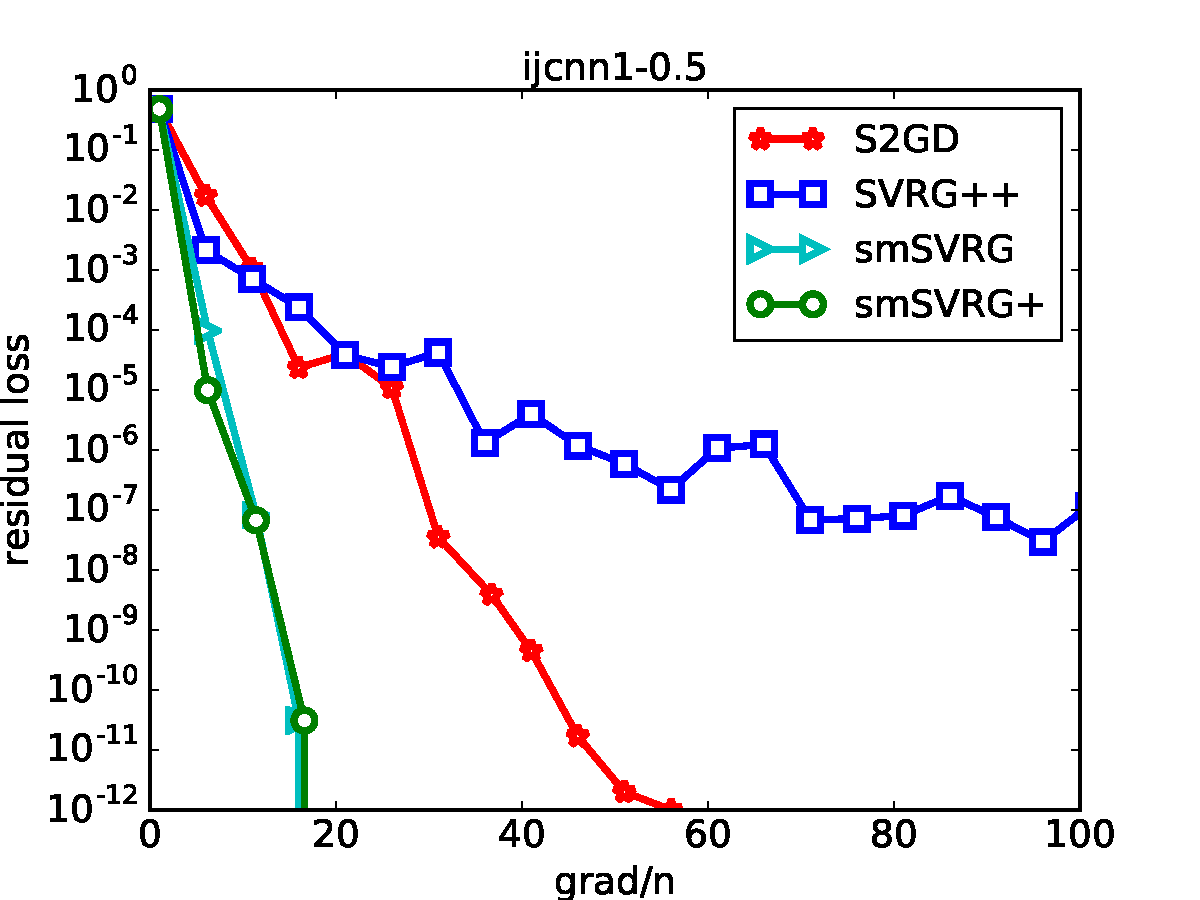
\includegraphics[width=0.24\linewidth]{cmijcnn105}\label{cmijcnn105}}
%\subfigure[ijcnn1 $\eta=0.05$]{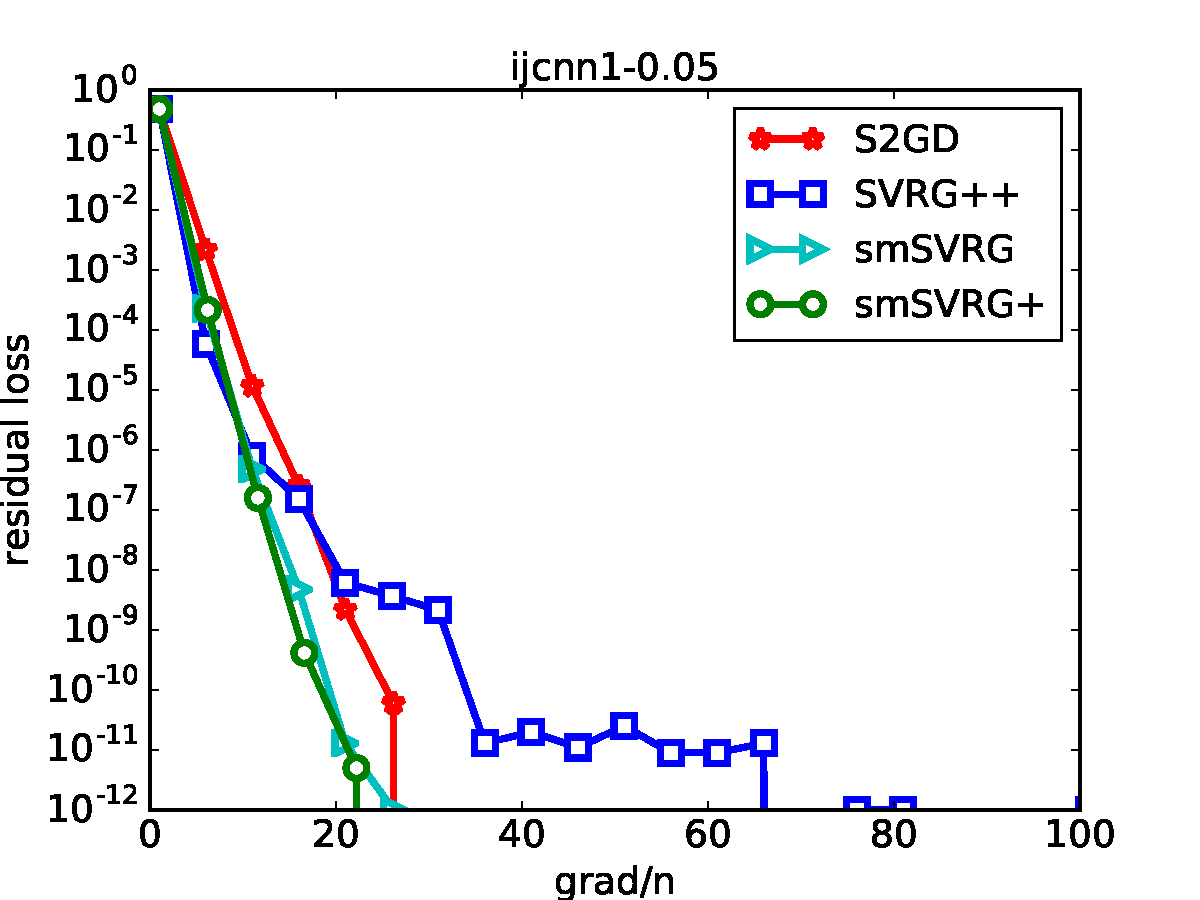
\includegraphics[width=0.24\linewidth]{cmijcnn1005}\label{cmijcnn1005}}
%\subfigure[ijcnn1 $\eta=0.01$]{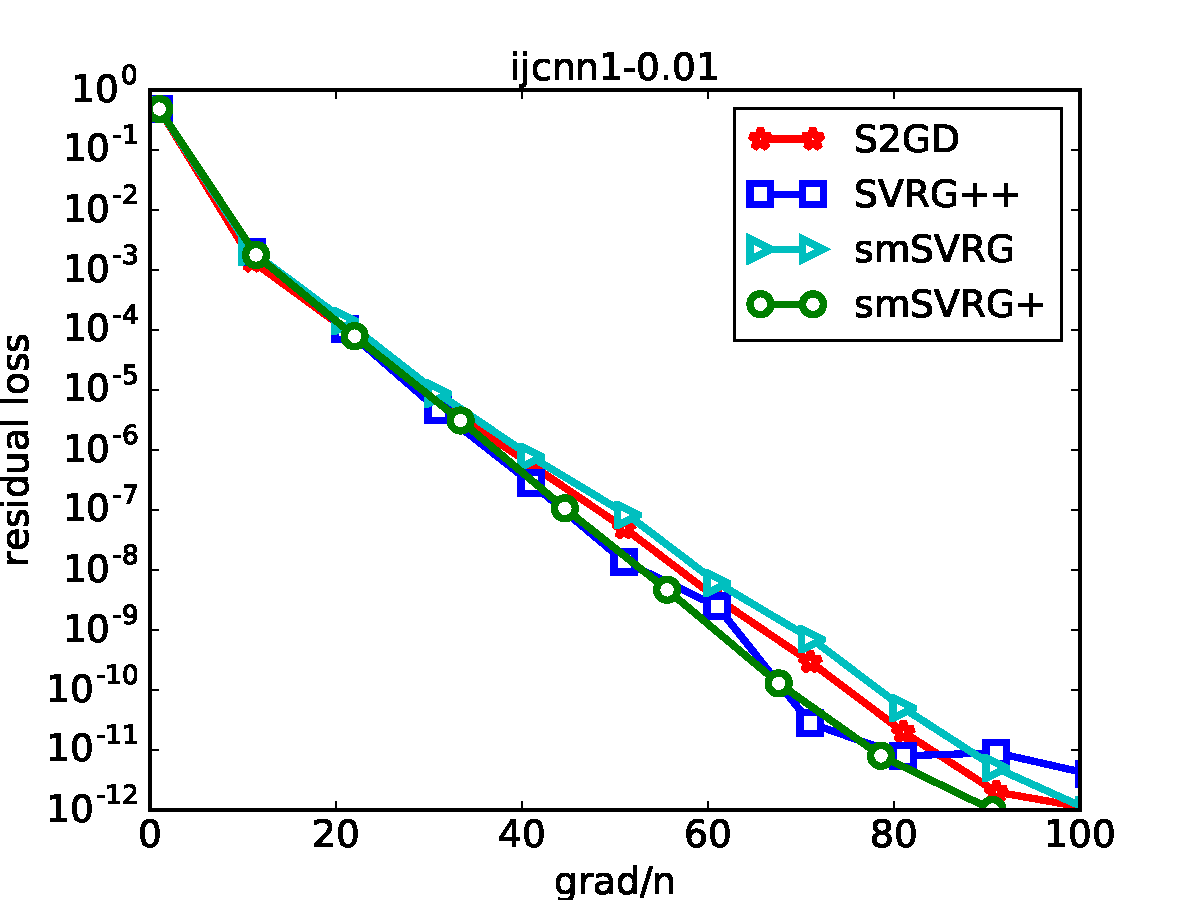
\includegraphics[width=0.24\linewidth]{cmijcnn1001}\label{cmijcnn1001}}
%\subfigure[ijcnn1 $\eta=0.001$]{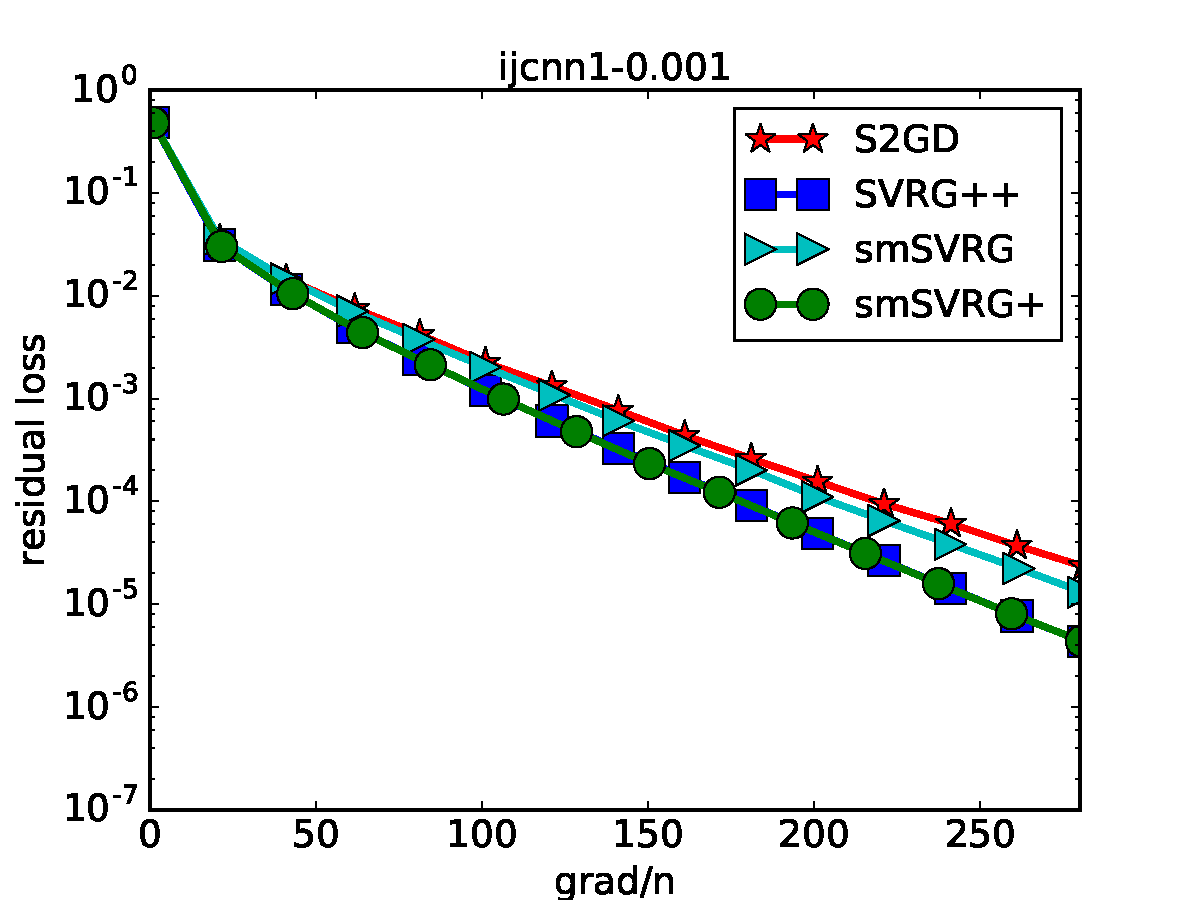
\includegraphics[width=0.24\linewidth]{cmijcnn10001}\label{cmijcnn10001}}
%\label{cmijcnn1}
%\caption{Comparison of \textsc{smSVRG}, \textsc{smSVRG+}, SVRG++, S2GD}
%\end{figure*}
 \begin{figure*}[htb]
\centering
\subfigure[w8a $\eta=0.1$]{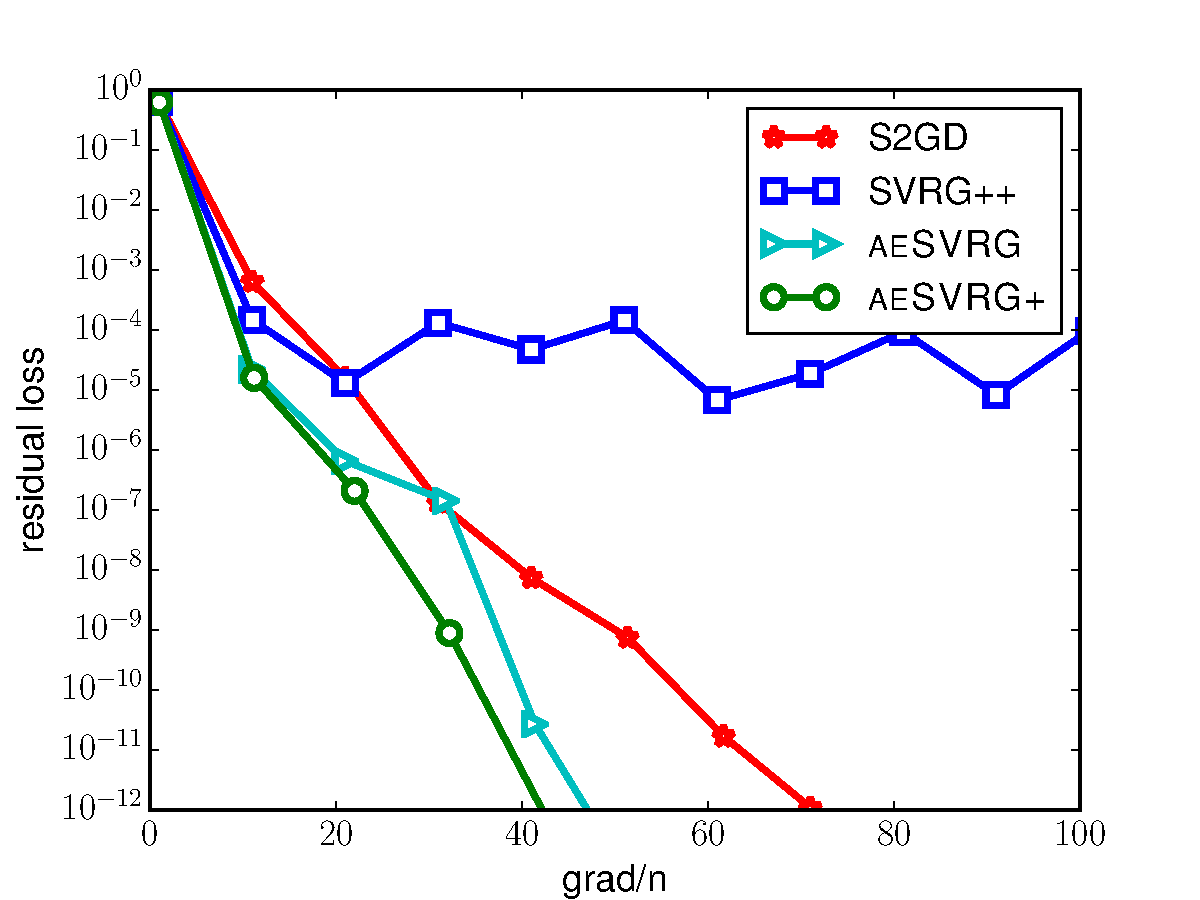
\includegraphics[width=0.5\columnwidth]{cm_w8a01}\label{cm_w8a01}}
\subfigure[mushrooms $\eta=0.1$]{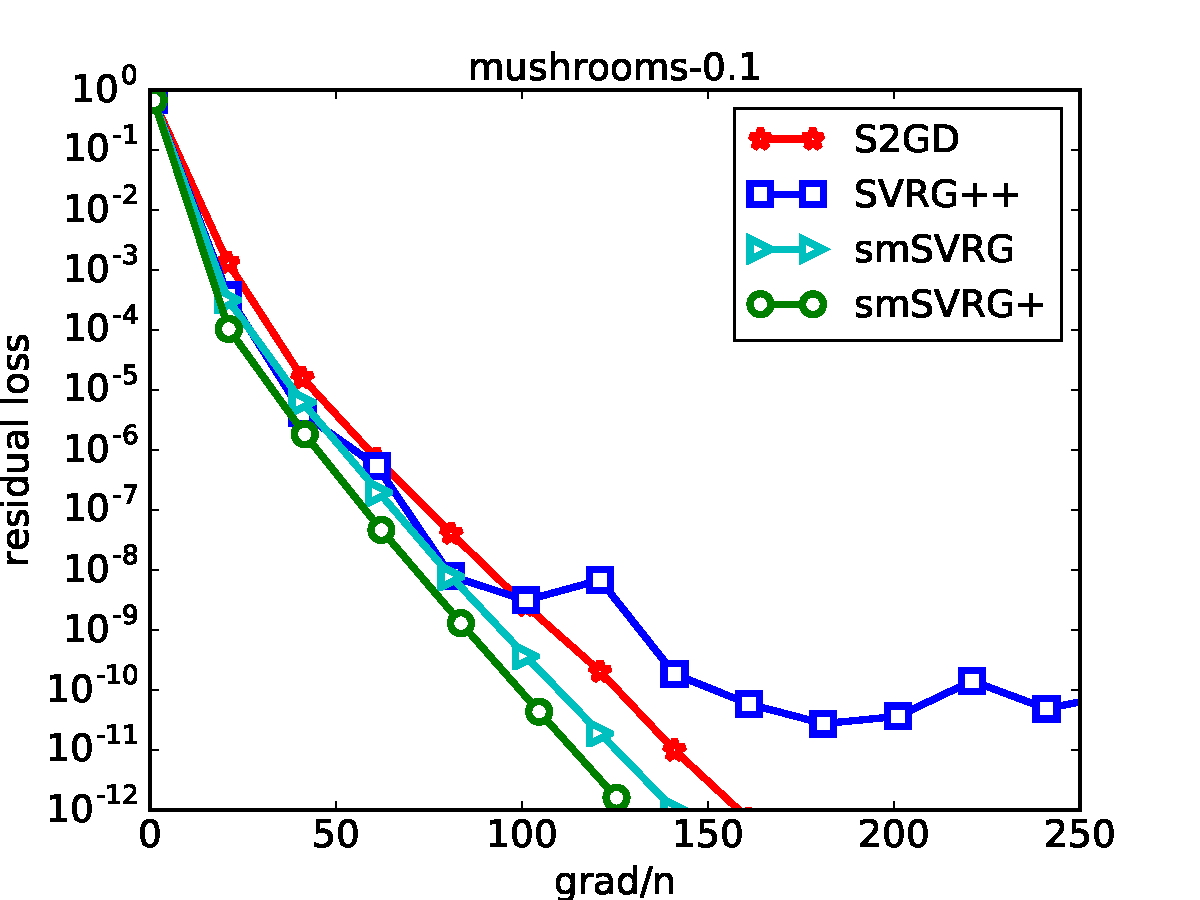
\includegraphics[width=0.5\columnwidth]{cm_mushrooms01}\label{cm_mushrooms}}
\subfigure[abalone $\eta=0.1$]{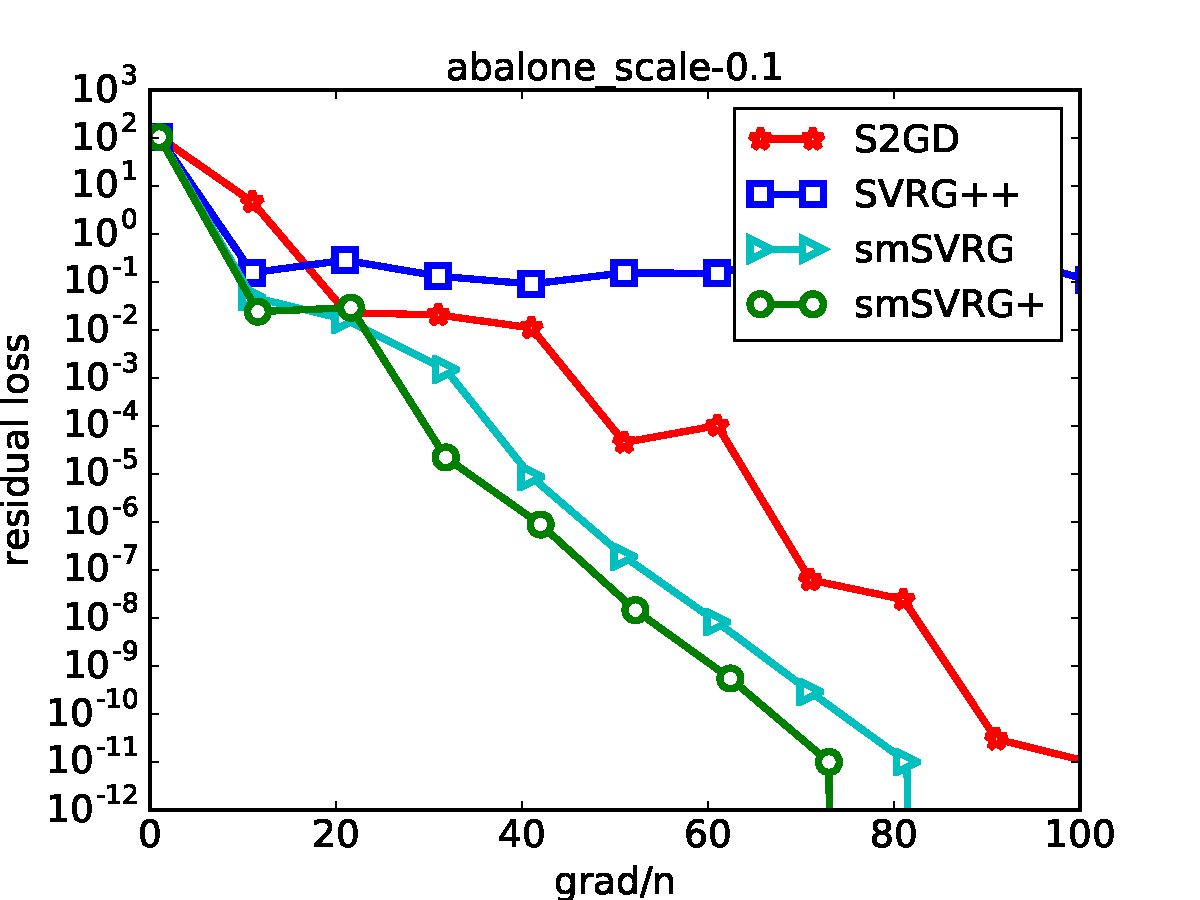
\includegraphics[width=0.5\columnwidth]{cm_abalone_scale01}\label{cm_abalone01}}
\subfigure[mg $\eta=0.1$]{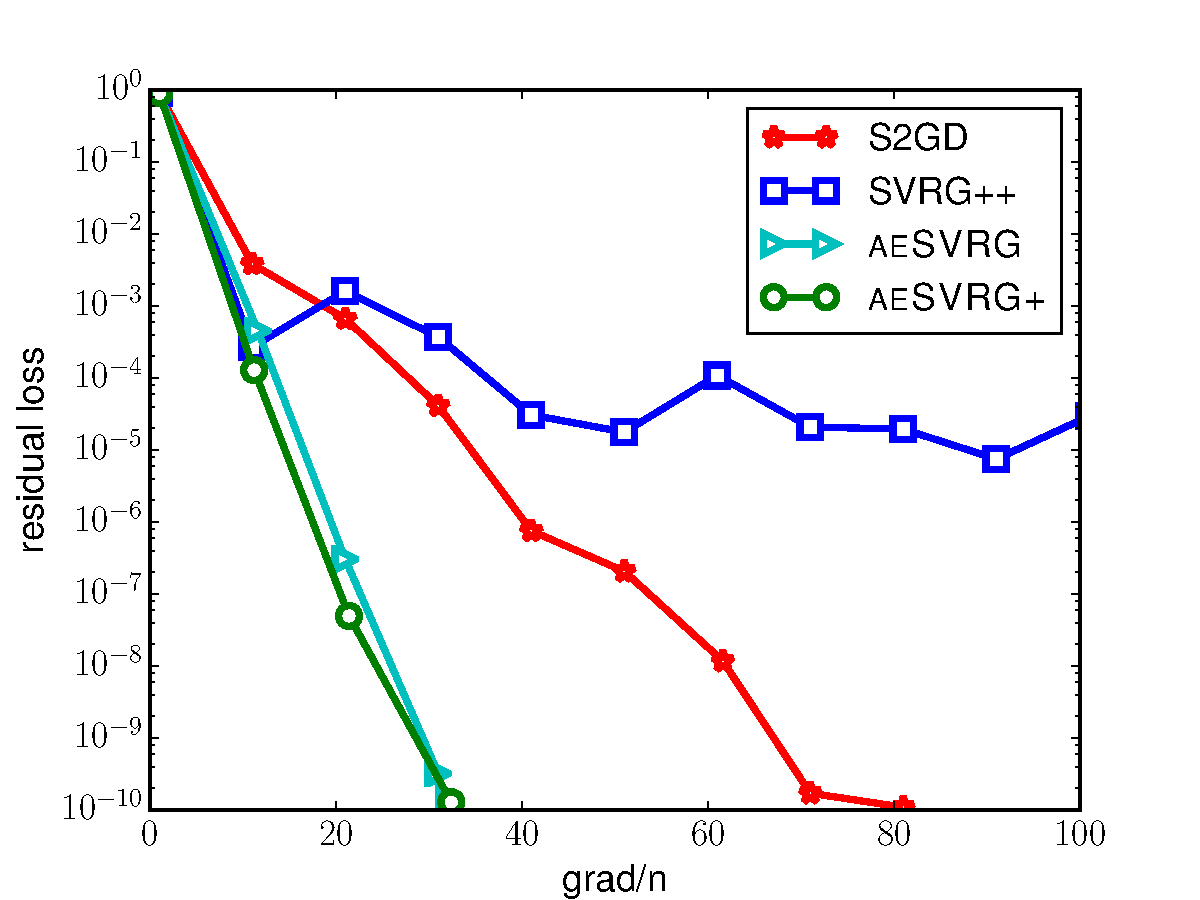
\includegraphics[width=0.5\columnwidth]{cm_mg_scale01}\label{cm_mg01}}
\caption{Comparison of \textsc{smSVRG}, \textsc{smSVRG+}, SVRG++, S2GD on four datasets. }
\label{cm_test}
\end{figure*}





 
 \section{Numerical Experiments}
 \label{numexperiments}
 %\subsection{Experimental settings}
 In this section, we conduct some experiments to demonstrate the efficiency of our proposed algorithm. We evaluate our algorithm on eight training datasets, which are public on the LIBSVM website\footnote{http://www.csie.ntu.edu.tw/$\sim$cjlin/libsvmtools/datasets/}. In our experiments, algorithms are applied for two standard machine learning tasks: $l2$-regularized logistic regression and $l2$-regularized ridge regression.
 
 The $l2$-regularized logistic regression task is conducted on the two datasets: ijcnn1, a9a, w8a and mushrooms. Since the label of each instance in these datasets is set to be 1 or -1, the loss function of $l2$-regularized logistic regression task is:
\begin{equation}
\label{logistic_reg}
\min\limits_\omega \frac{1}{n}\sum\limits_{i=1}^n \log(1+e^{-y_i \omega^\mathrm{T} x_i }) + \lambda \parallel \omega \parallel^2.
\end{equation}
The $l2$-regularized ridge regression task is conducted on the four datasets: YearPredictMSD, cadata, mg, abalone. The loss function of $l2$-regularized ridge regression task is:
\begin{equation}
\label{ridge_reg}
\min\limits_\omega \frac{1}{n}\sum\limits_{i=1}^n\left(\omega^{\mathrm{T}}x_i-y_i\right)^2 + \lambda \parallel \omega \parallel^2.
\end{equation}
We scale the value of all features to $[-1,1]$ and set the weighting parameter $\lambda$ to $10^{-4}$ for all evaluations. 
In all figures, the $x$-axis denotes the computational cost, which is measured by the number of gradient computation divided by the size of training data, i.e. $n$. The $y$-axis denotes training loss residual, i.e. $F(\tilde{\omega}_s) - F(\omega^{*})$. Note that the optimum $\omega^*$ is estimated by running the gradient descent for a long time. Our numerical experiments include three parts: comparing with existing related methods, comparing with SVRG by varying learning rate and sensitivity test on $m_0$. The experiments show the superior performance of our methods. 

\begin{table}[]
\centering
\caption{Detail information of datasets and models}
\label{data information}
\begin{tabular}{|l|l|l|l|l|}
\hline
Dataset           & size & dimension & model & $\lambda$ \\ \hline
ijcnn1            &  49990 &  22 &   logistic    &  $10^{-4}$         \\
a9a               &   32561&123   &     logistic  &      $10^{-4}$     \\ 
YearPredictionMSD & 463715  &  90 &    linear  &      $10^{-4}$     \\
cadata              & 20640  &8   &     linear  &    $10^{-4}$       \\ \hline
\end{tabular}
\end{table}



\subsection{Comparing with existing related methods}
In this section, we compare our \textsc{smSVRG} and \textsc{smSVRG+} with two aforementioned existing methods: SVRG++ and S2GD. We do not compare with SVRG\_Auto\_Epoch in that we find its termination condition of epoch is never satisfied and keeps doing SGD iteration, resulting in nonconvegence. For SVRG++, we initialize $m = n$. For S2GD, we set the maximum of $m$ to be $4n$. For both \textsc{smSVRG} and \textsc{smSVRG+}, we set the window size, i.e. $m_0$ to be $0.1n$. We evaluate these methods by running logistic regression on dataset ijcnn1. 
As illustrated in Figure \ref{cm_test}, we can see that SVRG++ always fluctuates violently and fails to converge due the large variance caused by too large epoch size. It is shown that \textsc{smSVRG} and \textsc{smSVRG+} always outperform SVRG++ and S2GD and converge rapidly. Besides, the performance of \textsc{smSVRG+} is superior to that of \textsc{smSVRG}. The main reason is that \textsc{smSVRG+} can adjust the windows size to a suitable value adaptively.

\begin{figure*}[ht]
\centering
\subfigure[ijcnn1 $\eta=0.5$]{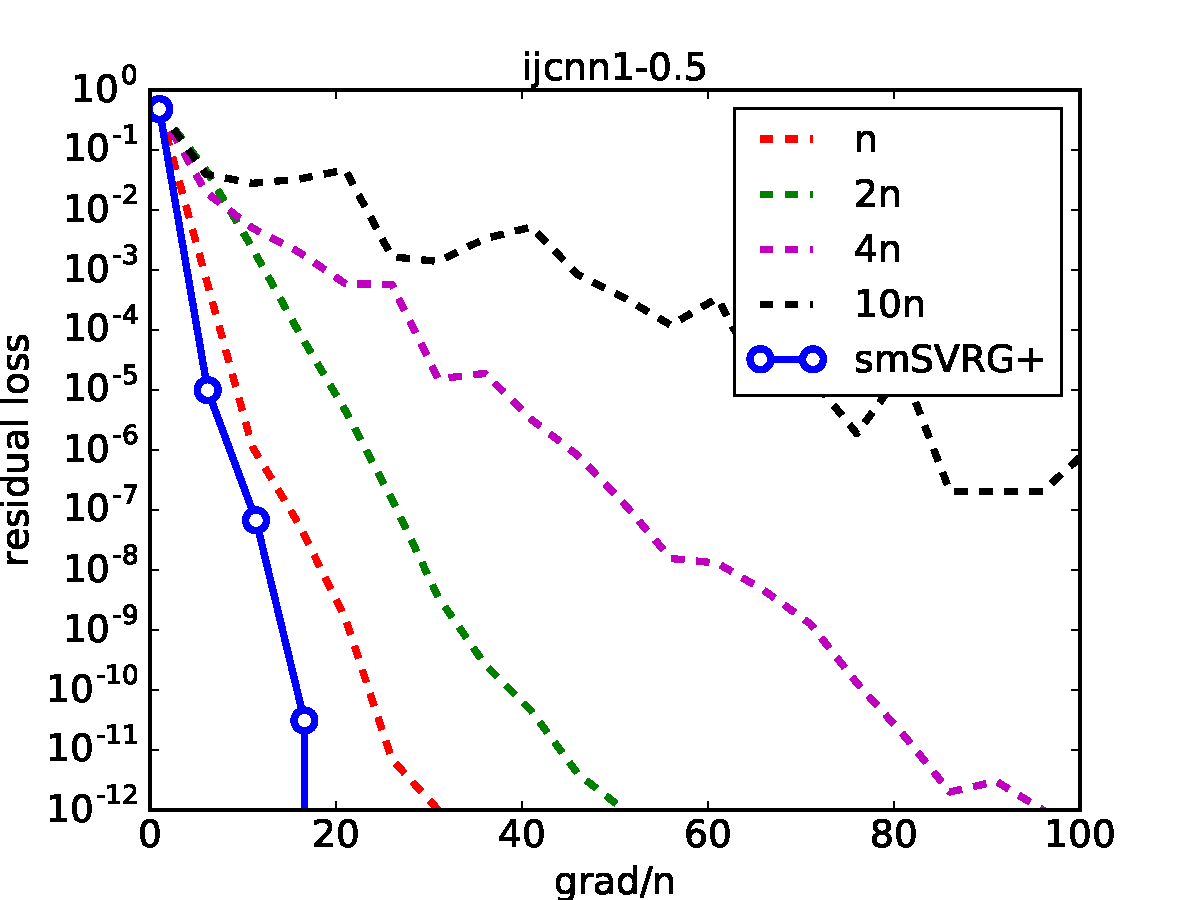
\includegraphics[width=0.5\columnwidth]{ijcnn105}\label{ijcnn105}}
\subfigure[ijcnn1 $\eta=0.05$]{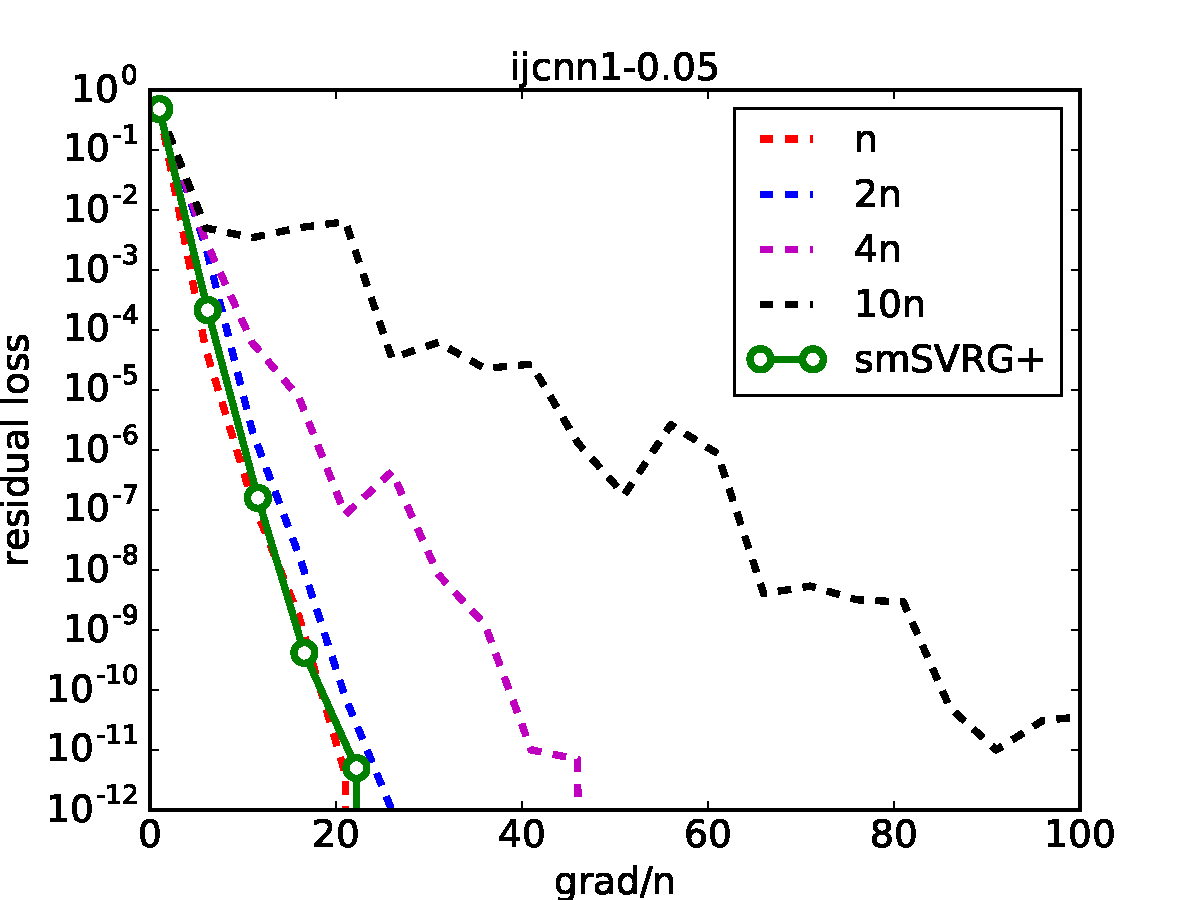
\includegraphics[width=0.5\columnwidth]{ijcnn1005}\label{ijcnn1005}}
\subfigure[ijcnn1 $\eta=0.01$]{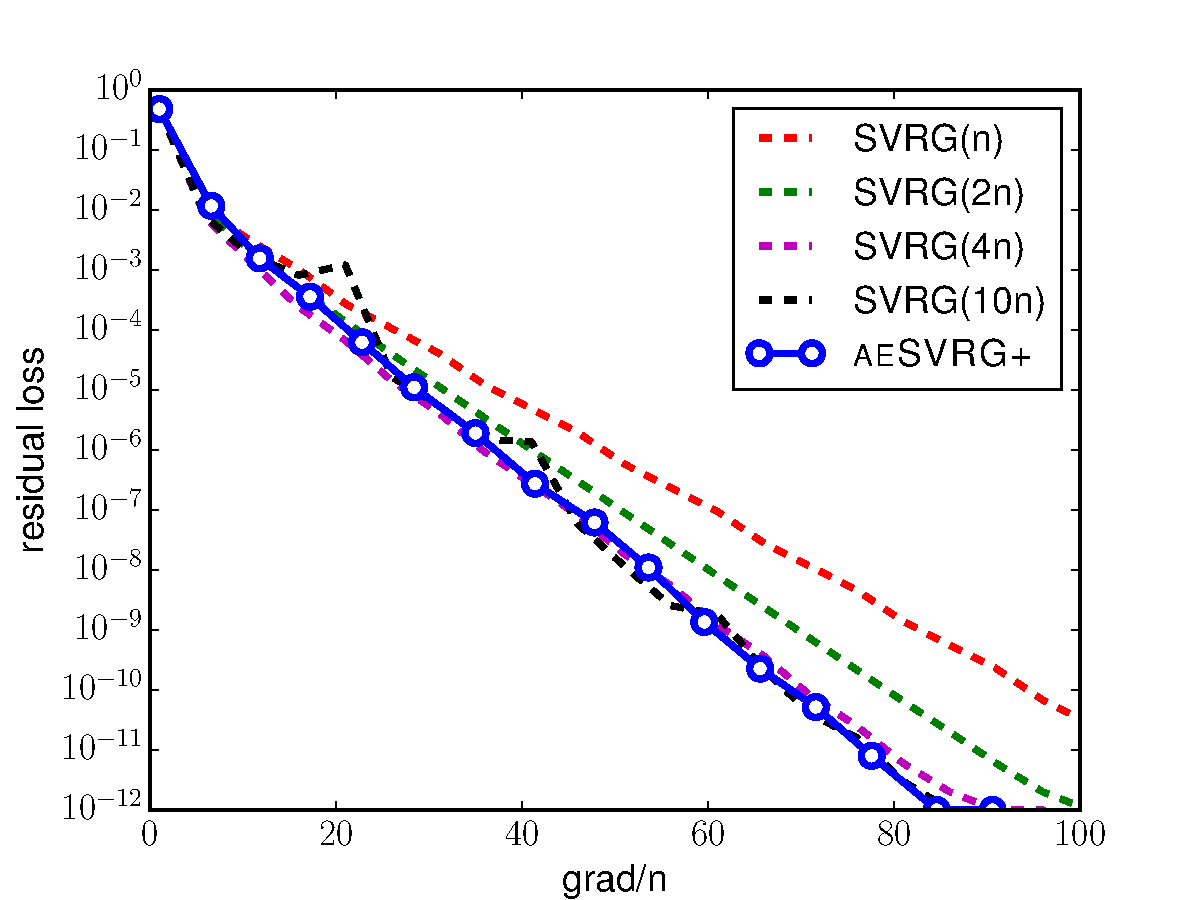
\includegraphics[width=0.5\columnwidth]{ijcnn1001}\label{ijcnn1001}}
\subfigure[ijcnn1 $\eta=0.001$]{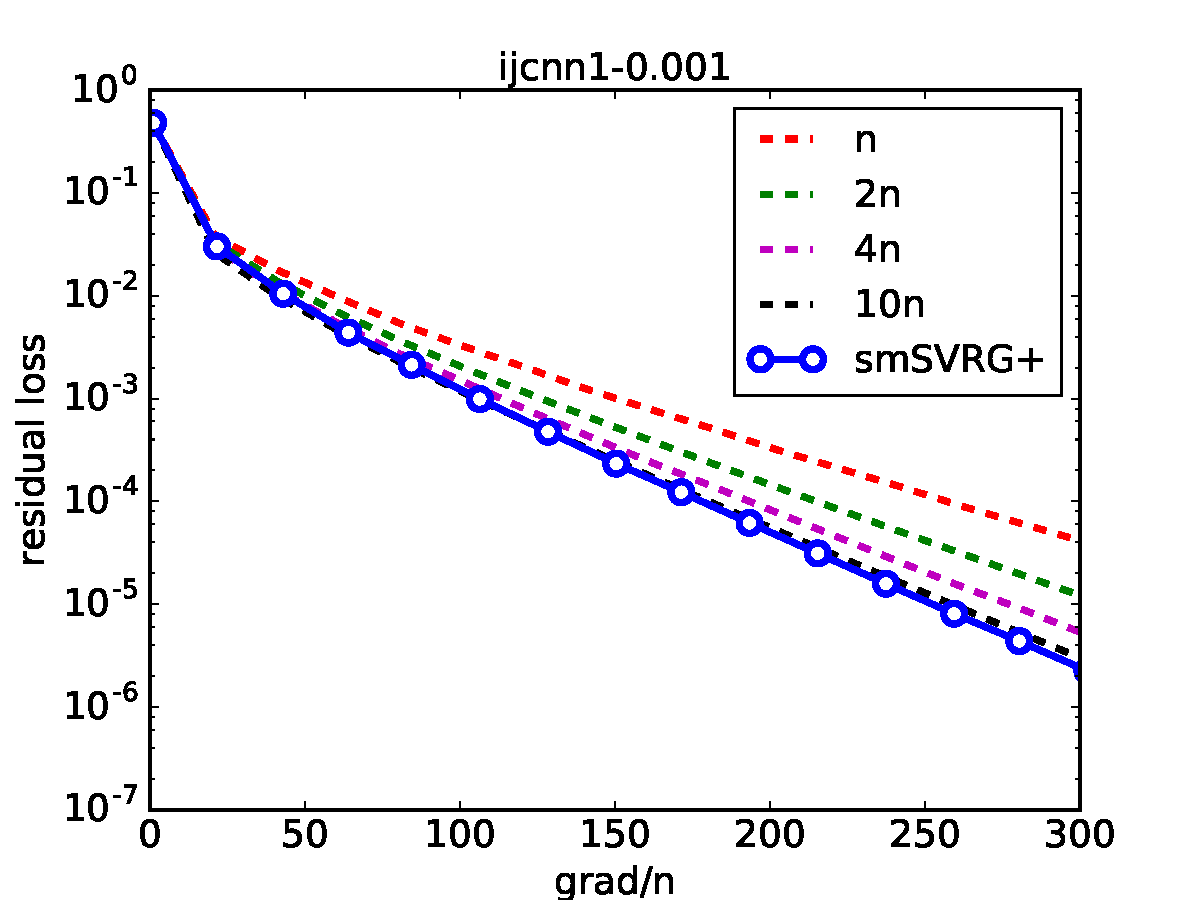
\includegraphics[width=0.5\columnwidth]{ijcnn10001}\label{ijcnn10001}}

\caption{Generally, \textsc{smSVRG} can automatically set an appropriate $m$ with different learning rates for the $l2$-regularized logistic regression}
\label{figure_logistic_ijcnn1}
\end{figure*}

\begin{figure*}[ht]
\centering
\subfigure[a9a $\eta=0.3$]{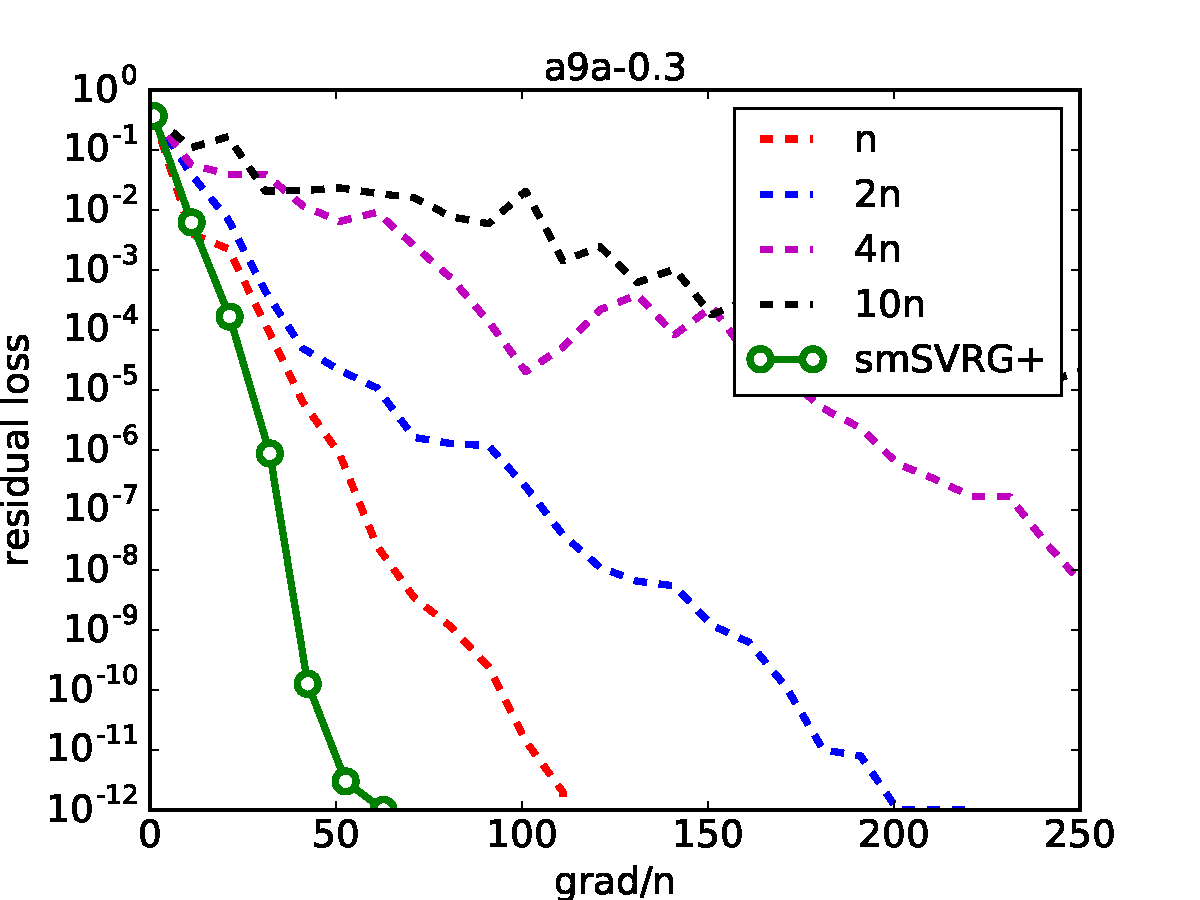
\includegraphics[width=0.5\columnwidth]{a9a03}\label{a9a03}}
\subfigure[a9a $\eta=0.05$]{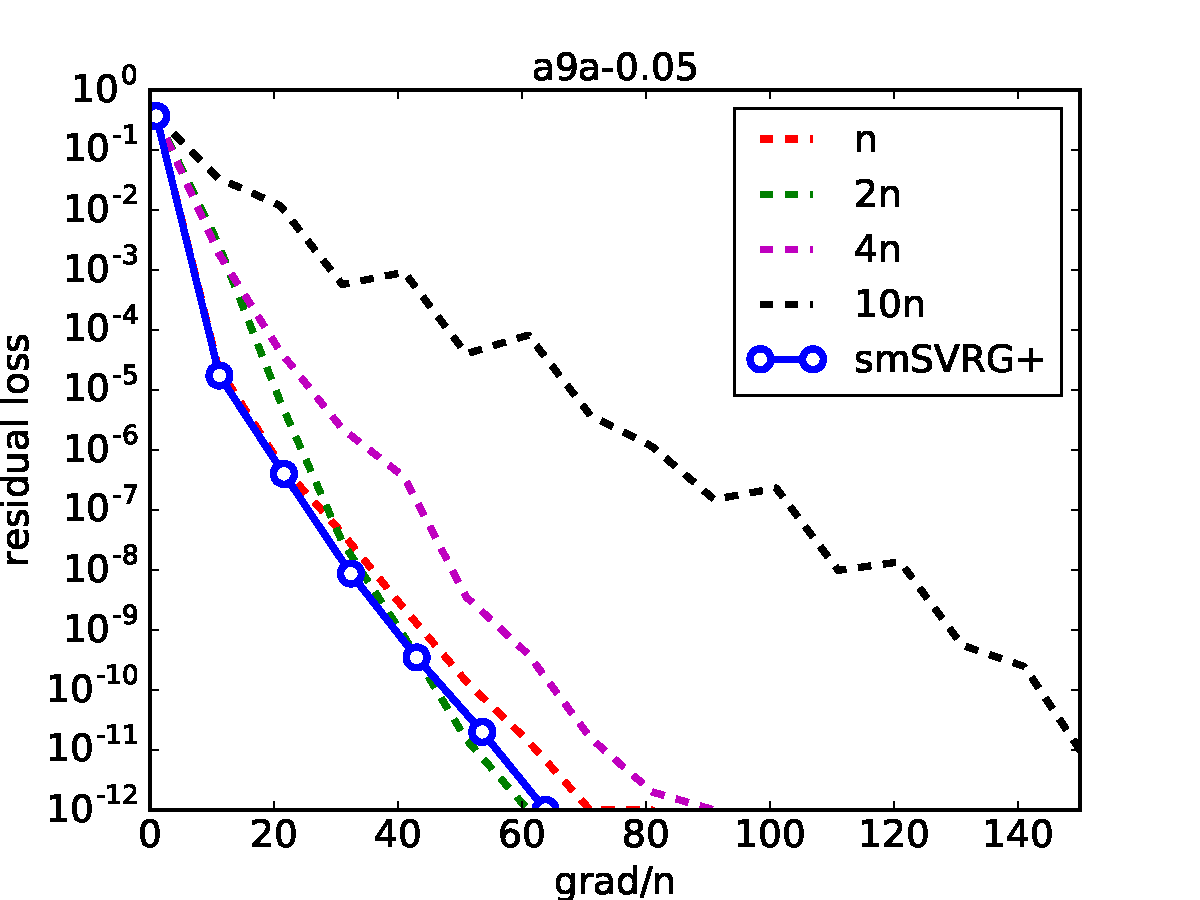
\includegraphics[width=0.5\columnwidth]{a9a005}\label{a9a005}}
\subfigure[a9a $\eta=0.02$]{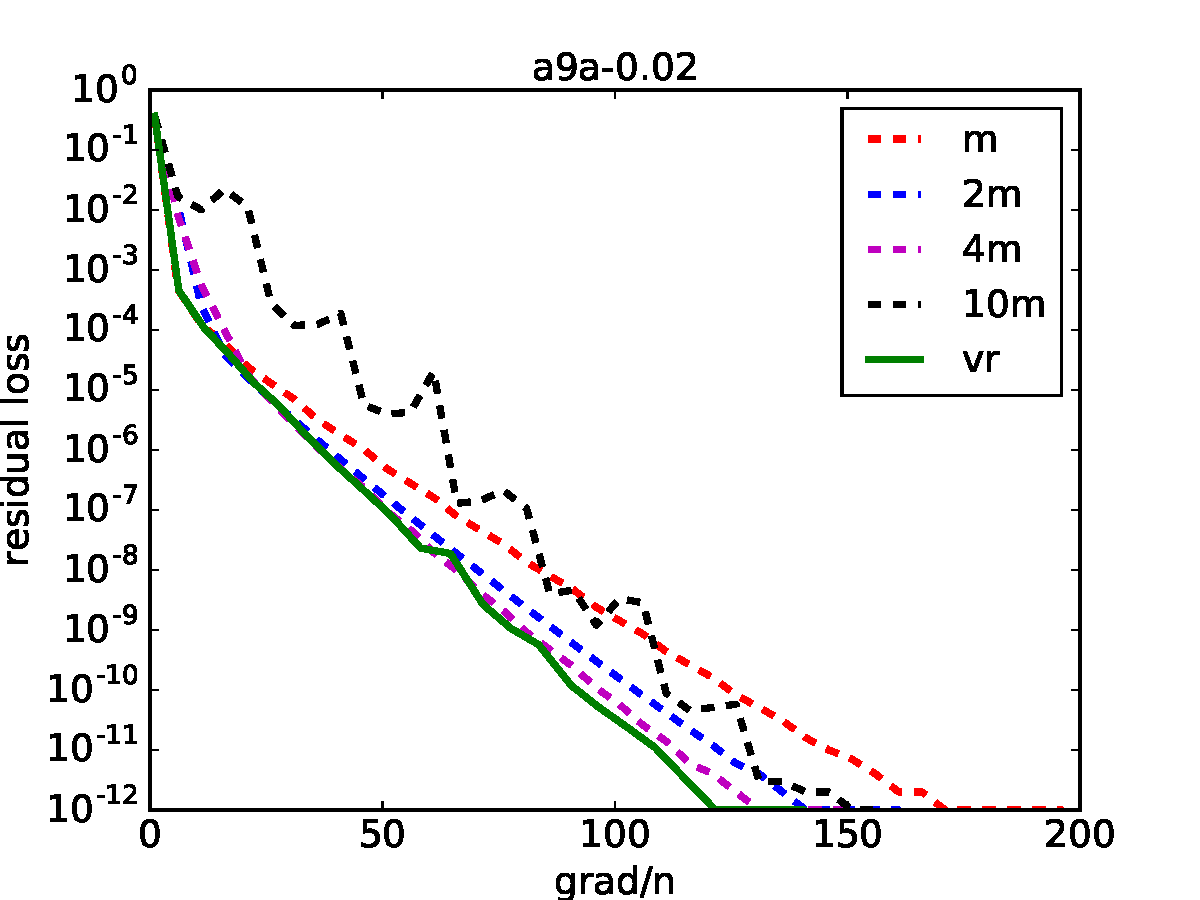
\includegraphics[width=0.5\columnwidth]{a9a002}\label{a9a002}}
\subfigure[a9a $\eta=0.001$]{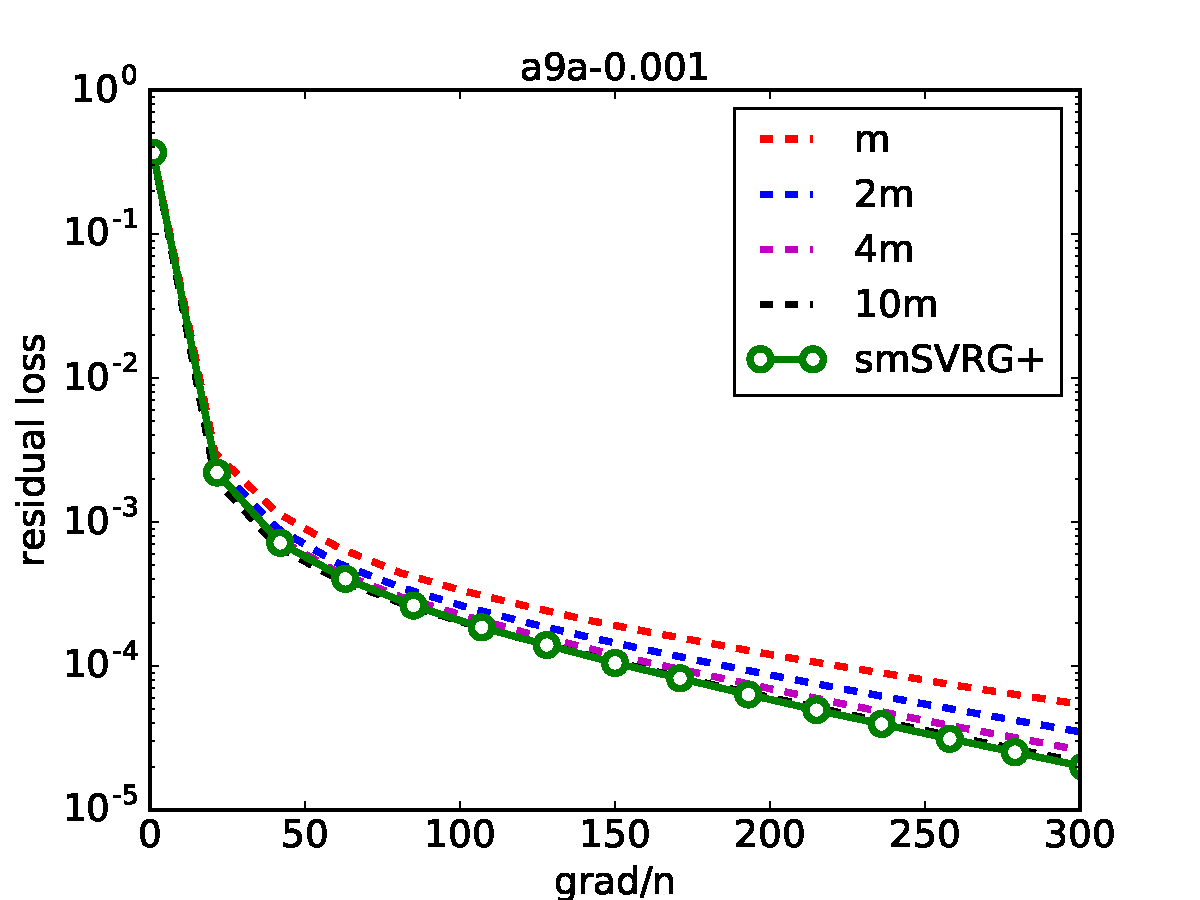
\includegraphics[width=0.5\columnwidth]{a9a0001}\label{a9a0001}}

\caption{Generally, \textsc{smSVRG} can automatically set an appropriate $m$ with different learning rates for the $l2$-regularized logistic regression}
\label{figure_logistic_a9a}
\end{figure*}

\begin{figure*}[ht]
\subfigure[YearPredictionMSD $\eta=0.01$]{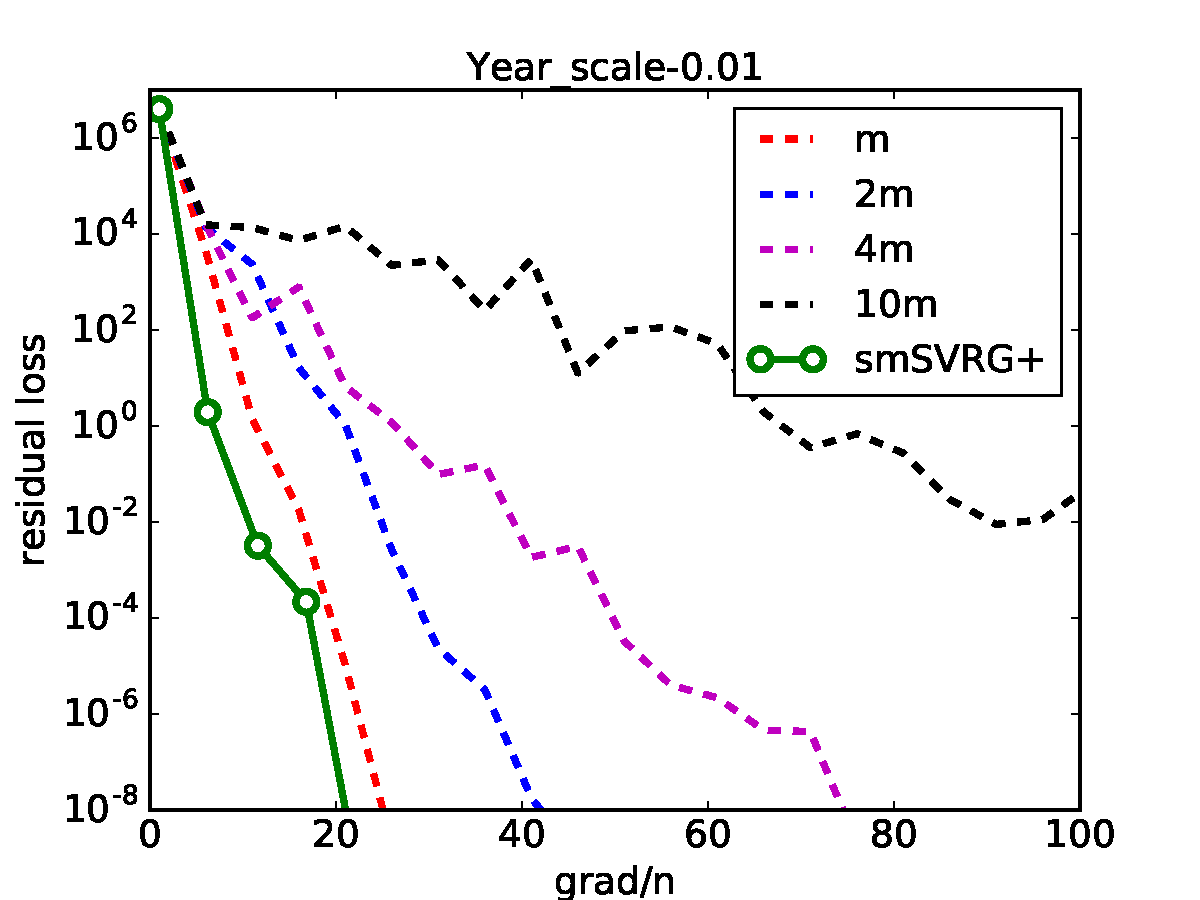
\includegraphics[width=0.5\columnwidth]{Year_scale001}\label{Year_scale001}}
\subfigure[YearPredictionMSD $\eta=0.005$]{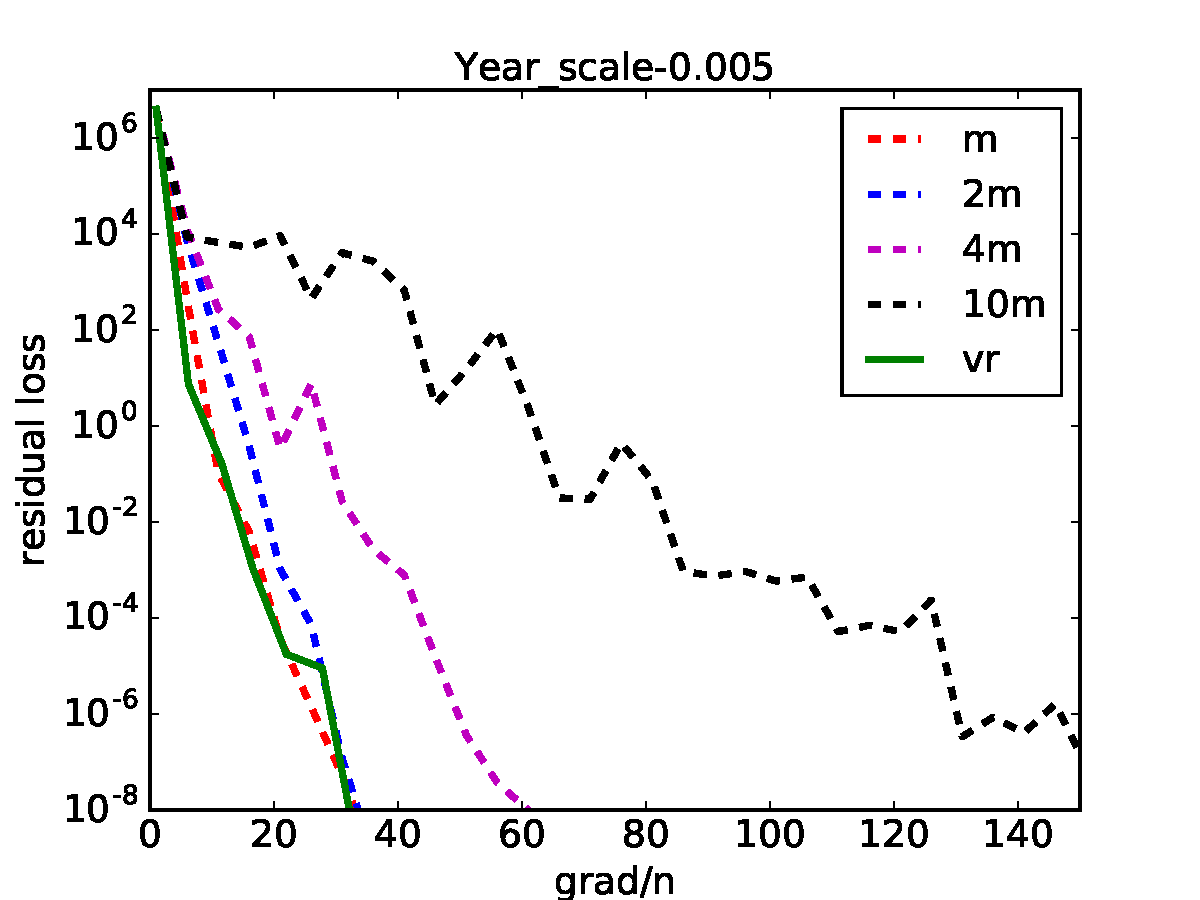
\includegraphics[width=0.5\columnwidth]{Year_scale0005}\label{Year_scale0005}}
\subfigure[YearPredictionMSD $\eta=0.002$]{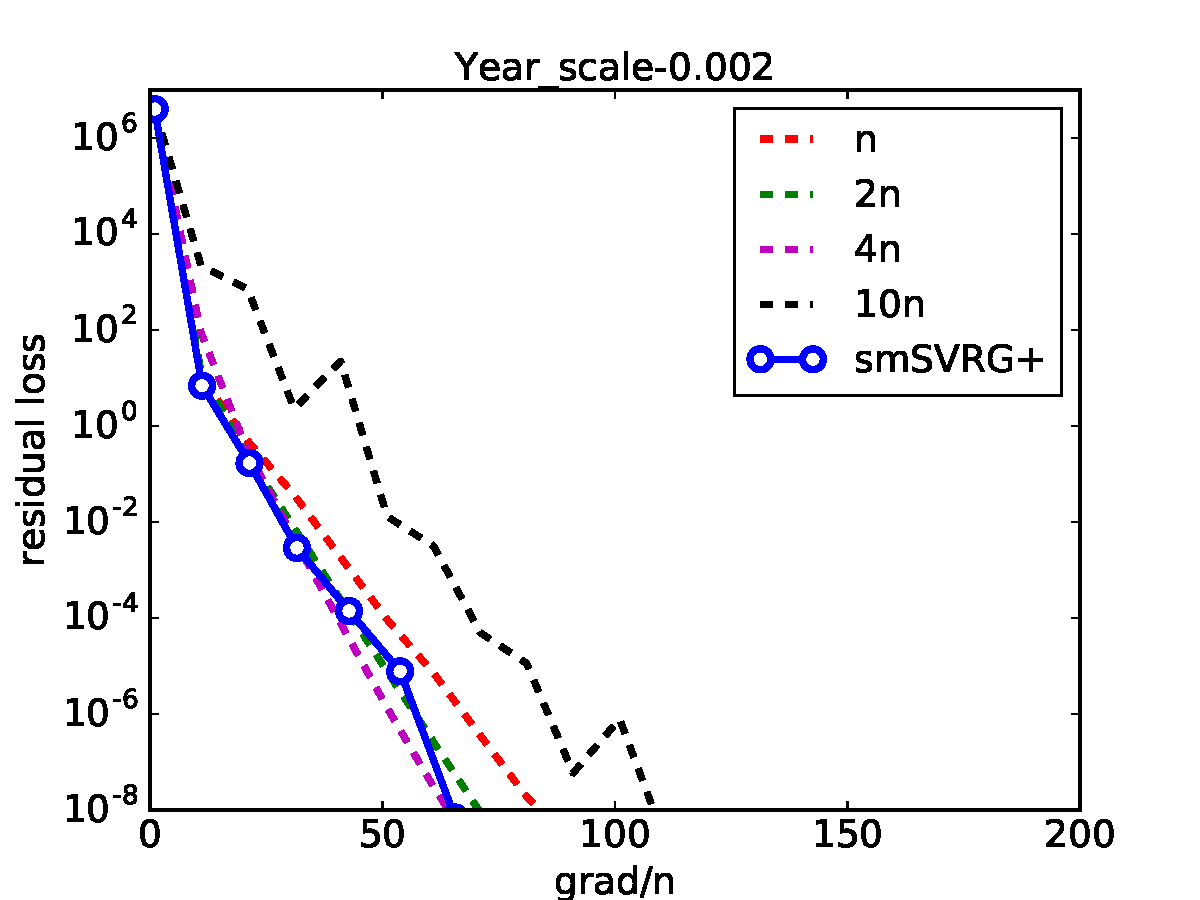
\includegraphics[width=0.5\columnwidth]{Year_scale0002}\label{Year_scale0002}}
\subfigure[YearPredictionMSD $\eta=0.0001$]{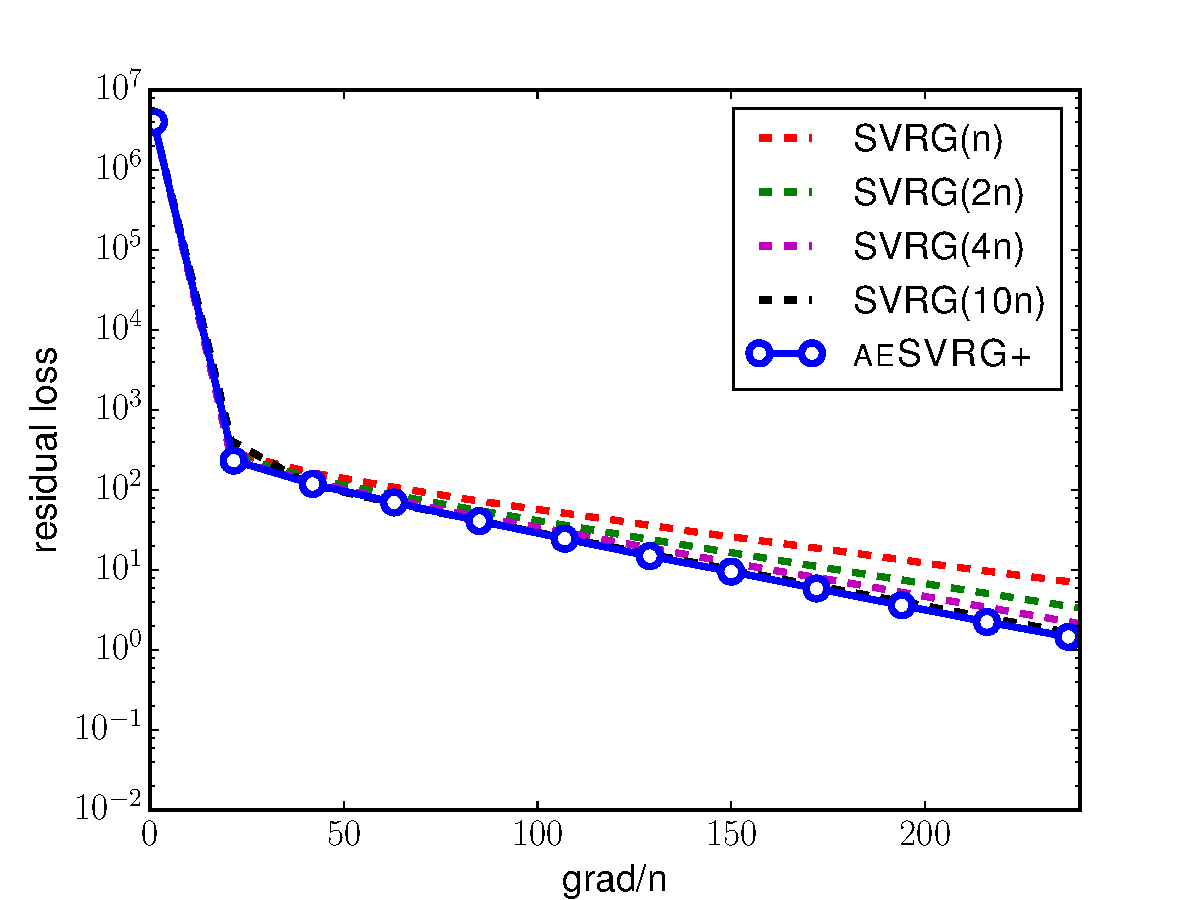
\includegraphics[width=0.5\columnwidth]{Year_scale00001}\label{Year_scale00001}}
\caption{Generally, \textsc{smSVRG} can automatically set an appropriate $m$ with different learning rates for the $l2$-regularized linear regression}
\label{figure_linear_Year}
\end{figure*}

\begin{figure*}[ht]
\subfigure[cadata $\eta=0.1$]{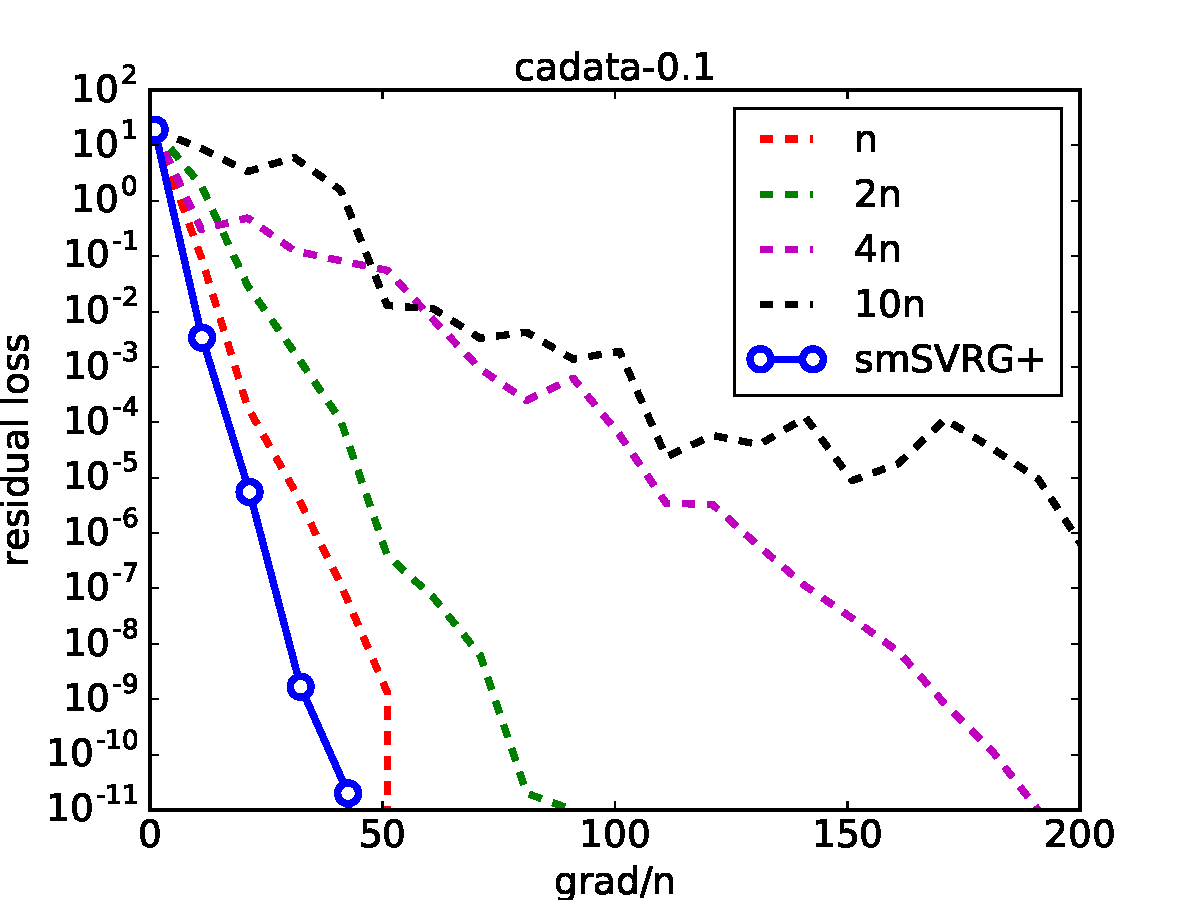
\includegraphics[width=0.5\columnwidth]{cadata01}\label{cadata01}}
\subfigure[cadata $\eta=0.05$]{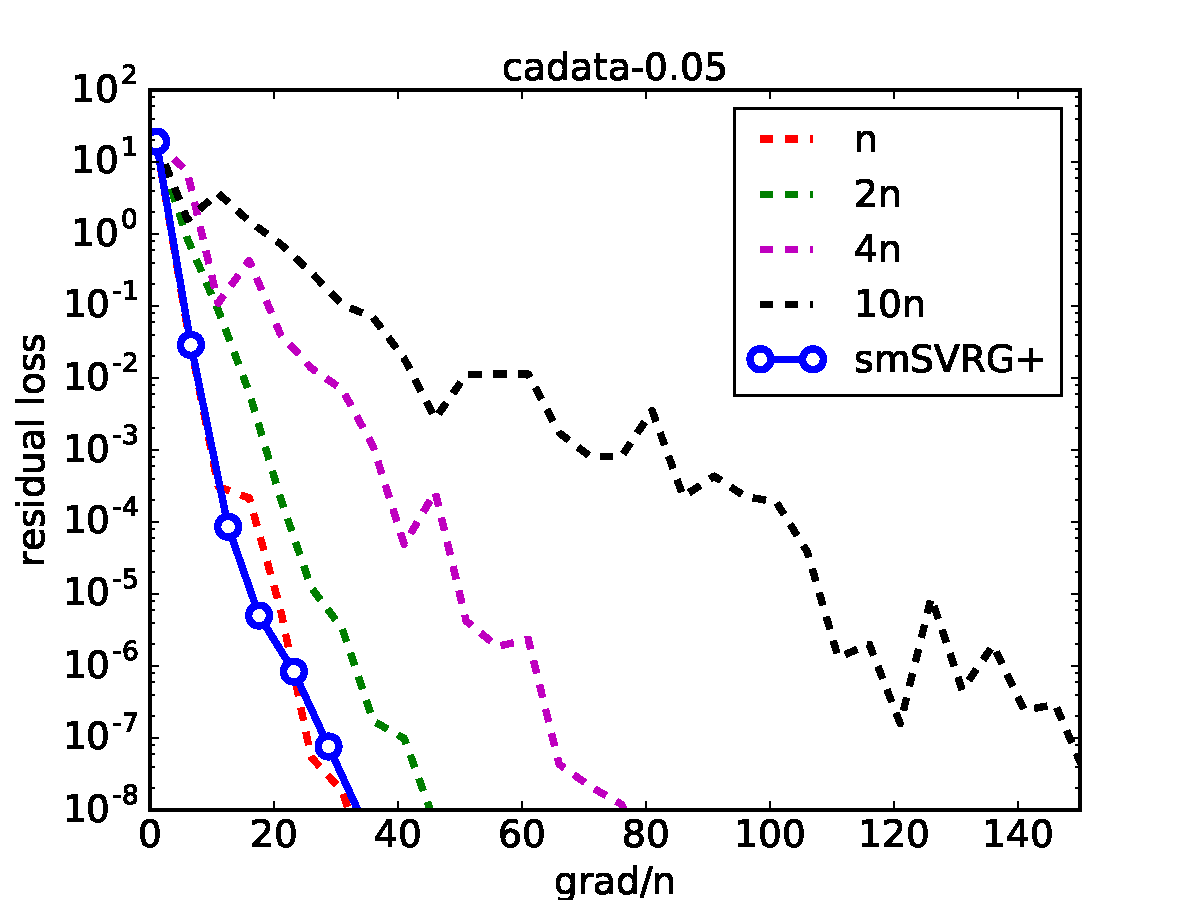
\includegraphics[width=0.5\columnwidth]{cadata005}\label{cadata005}}
\subfigure[cadata $\eta=0.02$]{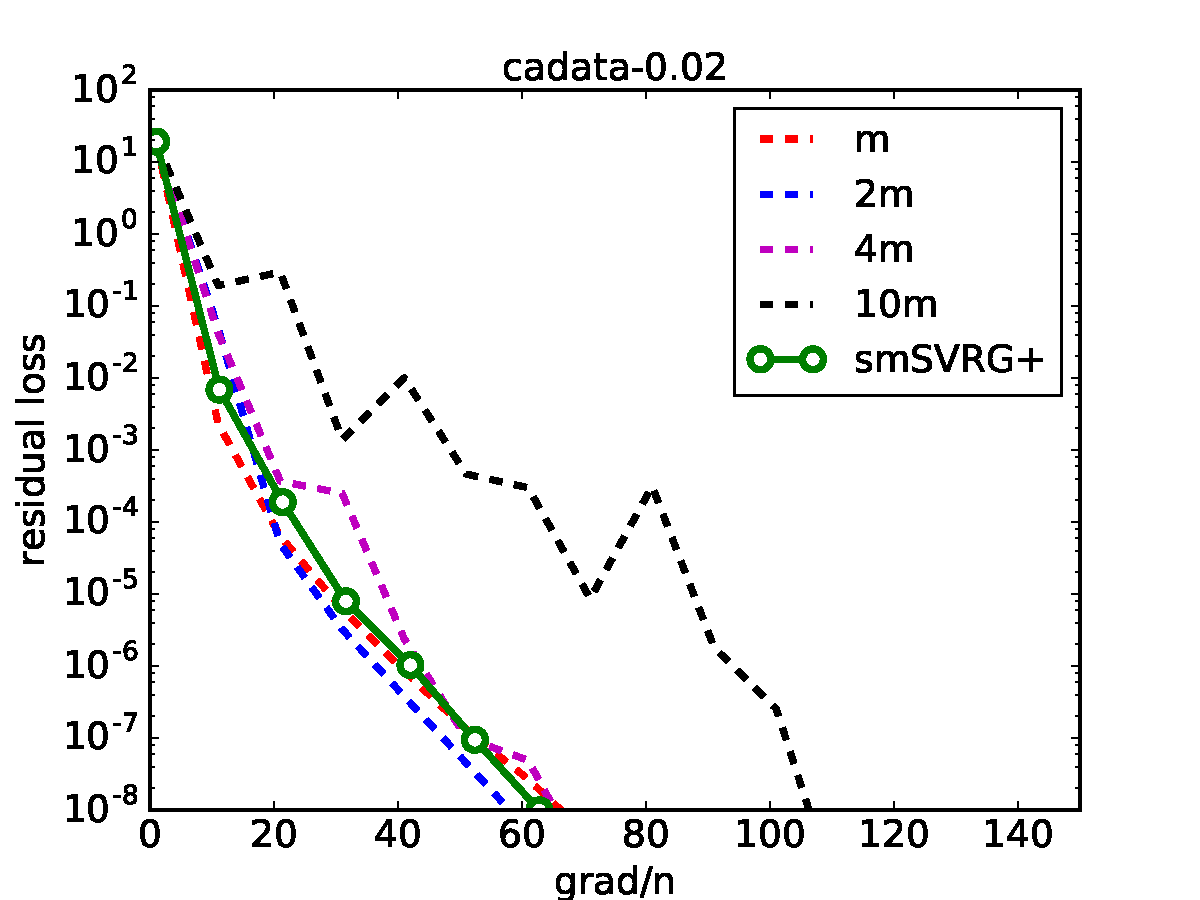
\includegraphics[width=0.5\columnwidth]{cadata002}\label{cadata002}}
\subfigure[cadata $\eta=0.001$]{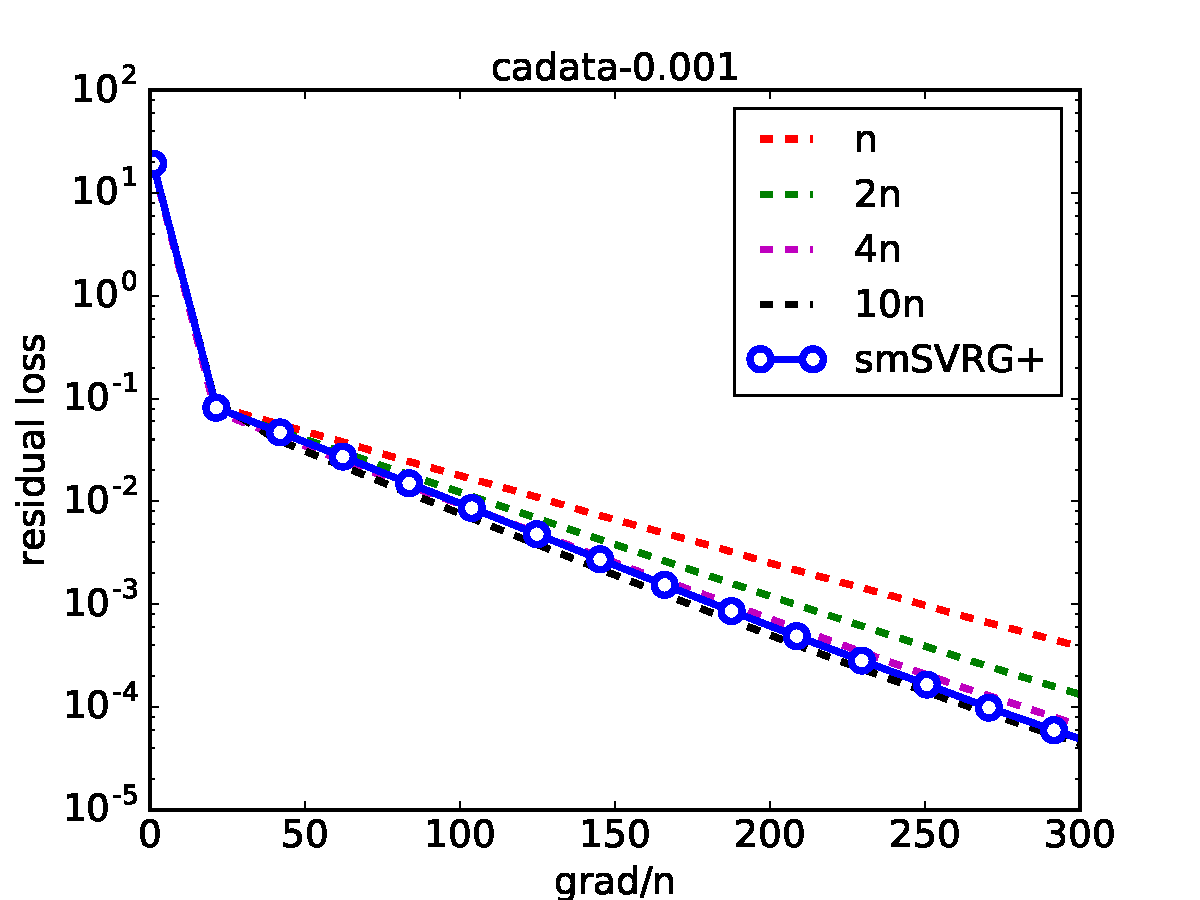
\includegraphics[width=0.5\columnwidth]{cadata0001}\label{cadata0001}}
\caption{Generally, \textsc{smSVRG} can automatically set an appropriate $m$ with different learning rates for the $l2$-regularized linear regression}
\label{figure_linear_cadata}
\end{figure*}


 \begin{figure*}[ht]
 \label{smSVRG_smSVRG+}
\centering
\subfigure[\textsc{smSVRG} on a9a]{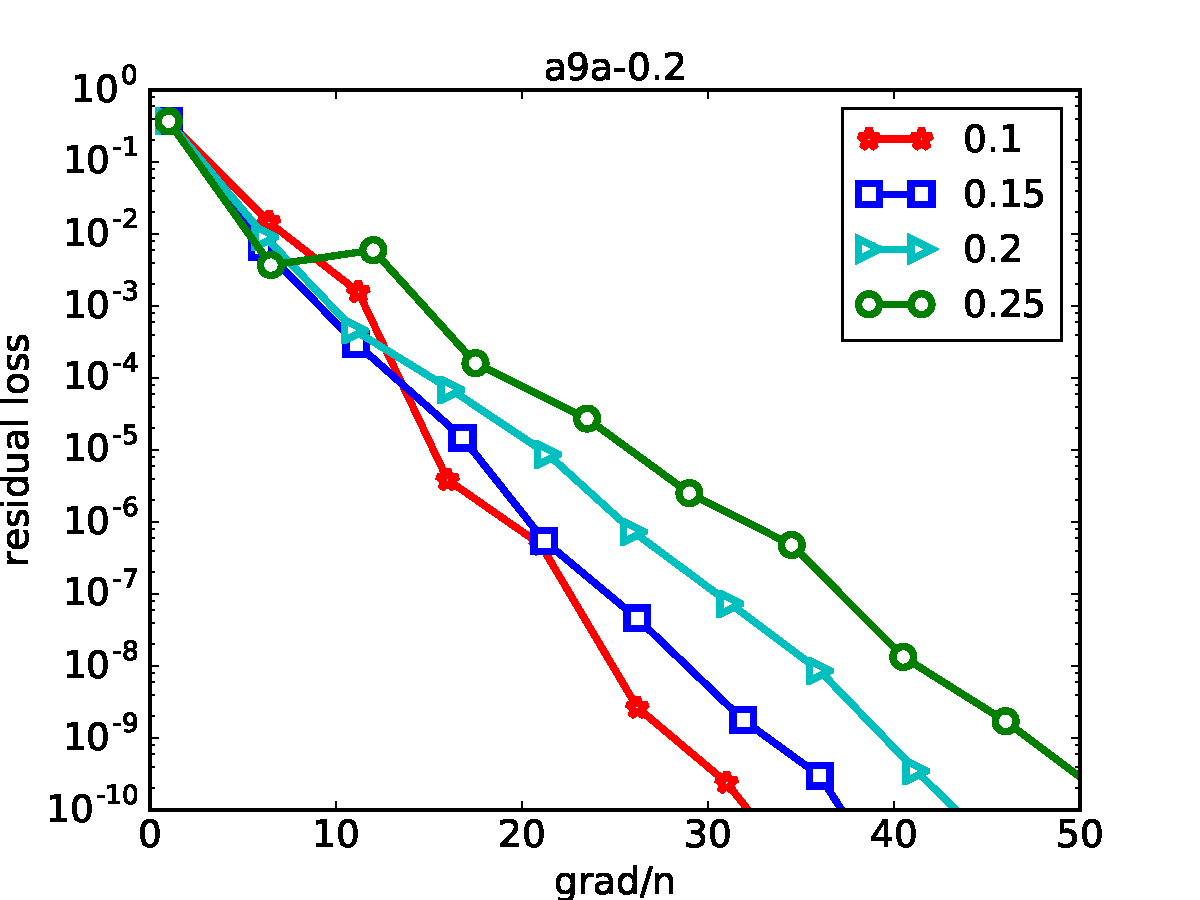
\includegraphics[width=0.5\columnwidth]{m0a9a02}\label{a9a_smSVRG}}
\subfigure[\textsc{smSVRG+} on a9a]{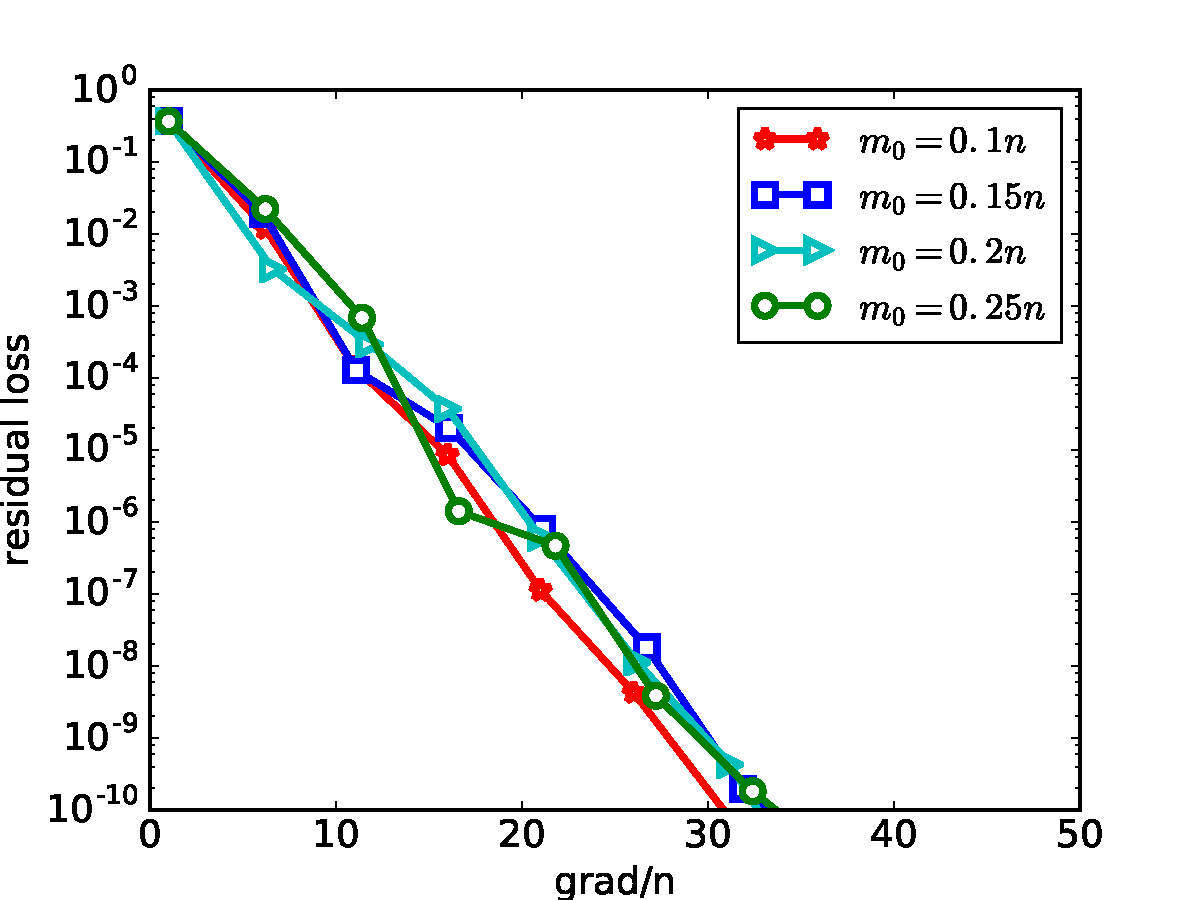
\includegraphics[width=0.5\columnwidth]{m0a9a02+}\label{a9a_smSVRG+}}
\subfigure[\textsc{smSVRG} on abalone]{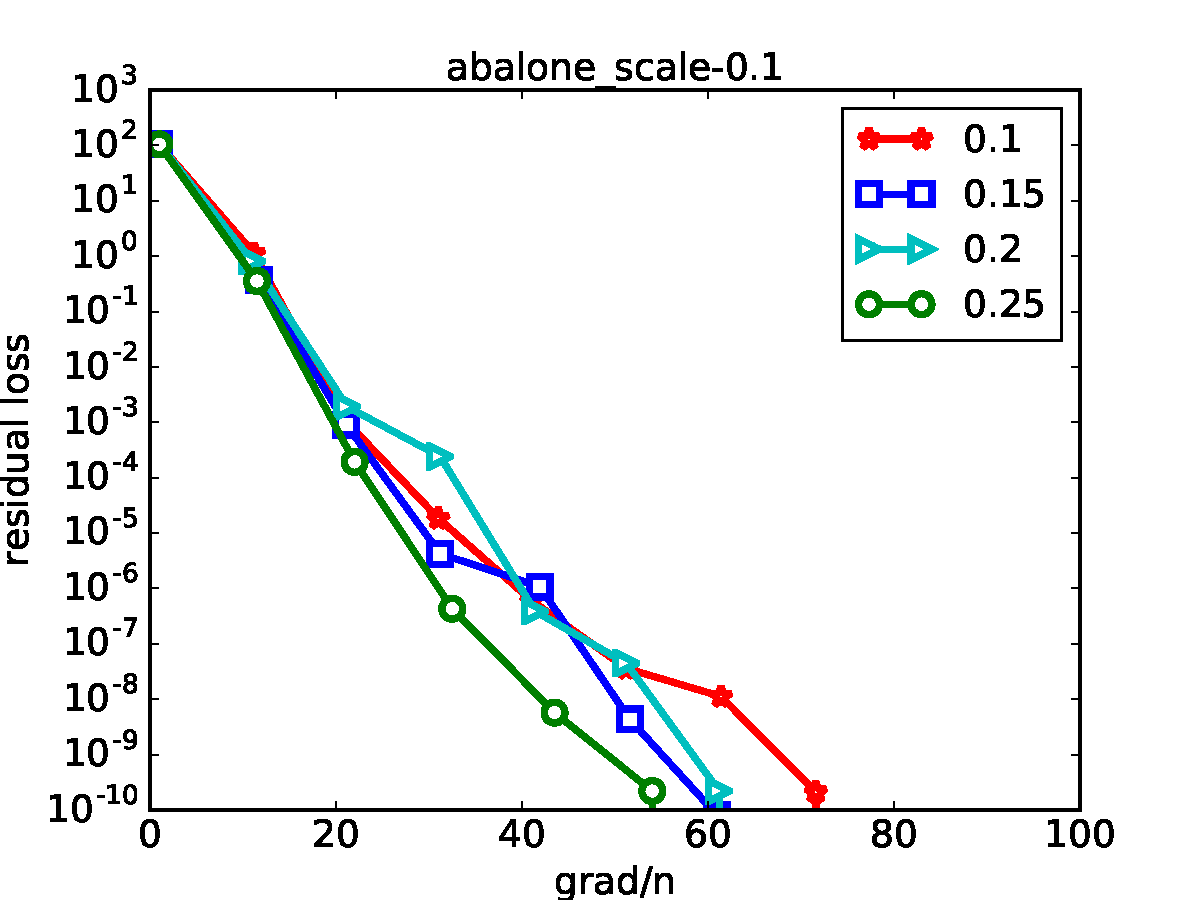
\includegraphics[width=0.5\columnwidth]{m0abalone_scale01}\label{abalone_smSVRG}}
\subfigure[\textsc{smSVRG+} on abalone]{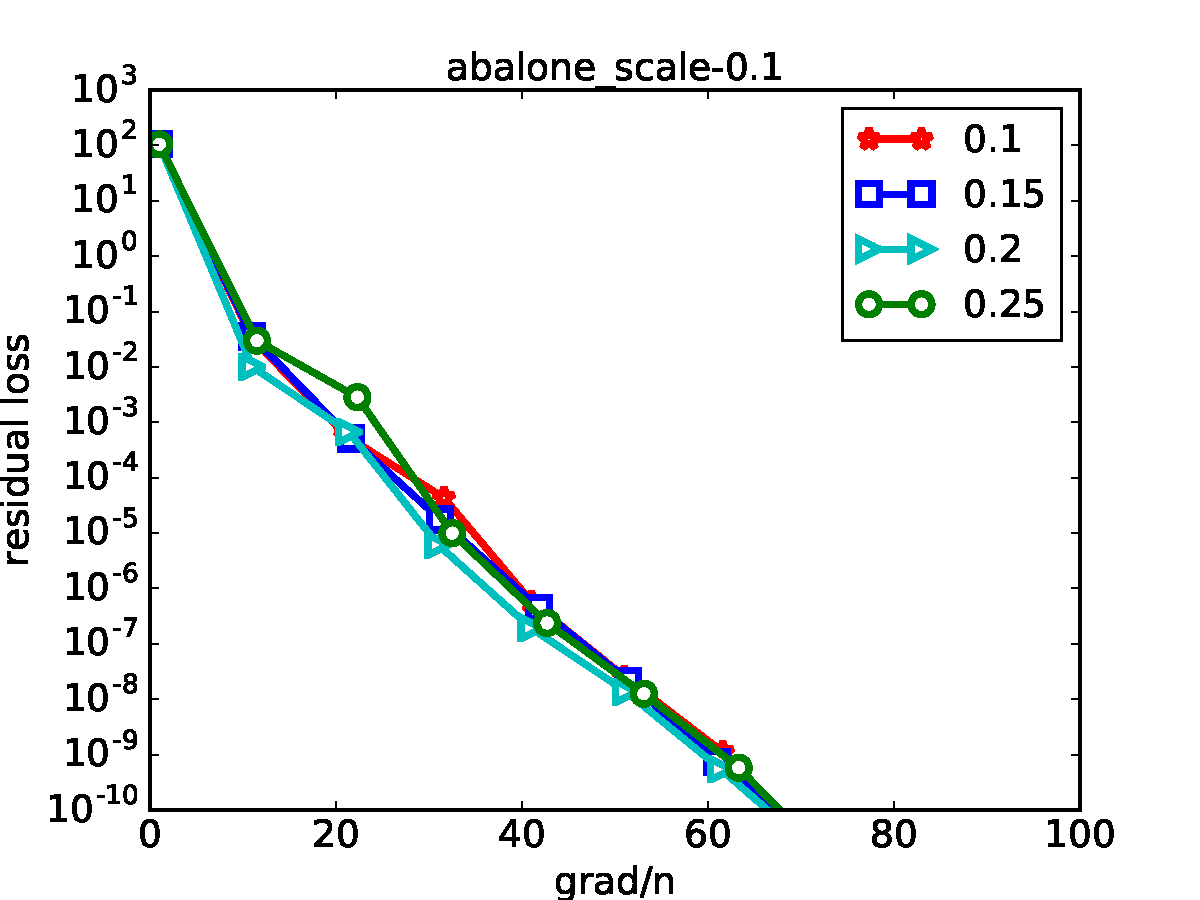
\includegraphics[width=0.5\columnwidth]{m0abalone_scale01+}\label{abalone_smSVRG+}}
\caption{Sensitivity test on $m_0$ for \textsc{smSVRG} and \textsc{smSVRG+}. The four numbers on the legends means four different choices of $m_0$. }

\end{figure*}

 \subsection{Comparing with SVRG by varying learning rate}
Since \textsc{smSVRG+} performs better than \textsc{smSVRG}, \textsc{smSVRG+} is used to conduct the comparison with SVRG. For SVRG, we increase the epoch size, i.e. $m$ as four different values: $n$, $2n$, $4n$, $10n$. The first three values are chosen because it is recommended to choose $m$ to be the same order of $n$ but slightly larger\citep{Johnson:9MAvkbgy}. Besides, our experiments show that epoch size larger than $10n$ have similar performance as the extremely large epoch size decrease the impact of full gradient computation. In all figures, the dashed lines represents SVRG with fixed epoch size; while the green solid lines stands for \textsc{smSVRG+}.

As illustrated in Figures \ref{figure_logistic_ijcnn1}, \ref{figure_logistic_a9a}, \ref{figure_linear_Year}, \ref{figure_linear_cadata},  \textsc{smSVRG+} can always have the similar performance as SVRG with most best-tuned epoch size. We observe that when $\eta$ is large,  and $m$ is set to be a small value, e.g. $n$, can achieve best performance. The main reason is that when $\eta$ is large, the variance becomes significant simultaneously, so $m$ must be set to be small in order to bound the variance. As $\eta$ decays, the optimal value of $m$ increases, which means that the algorithm can tolerate more variance induced by extra iterations. As illustrated in Figures \ref{ijcnn105}, \ref{a9a03}, \ref{Year_scale001}, \ref{cadata01}, our method is comparable to and sometimes even better than SVRG with best-tuned epoch sizes when learning rate is large or medium. However, As illustrated in Figures \ref{ijcnn10001}, \ref{a9a0001}, \ref{Year_scale00001}, \ref{cadata0001}, if $\eta$ is set to be too small, \textsc{smSVRG+} performs slightly inferior to  SVRG with large epoch sizes, but outperforms SVRG with recommended epoch sizes, i.e. $n$ and $2n$. It is noting that setting $\eta$ to be too small is not a practical approach when using SVRG or its variants, because the convergence rate will be extremely low. Therefore, the sub-optimal performance of \textsc{smSVRG+} with very small $\eta$ is acceptable.
 
\subsection{Sensitivity test on $m_0$}
In this section, we conduct the sensitivity test on both \textsc{smSVRG} and \textsc{smSVRG+} regarding window size $m_0$. As analyzed in \ref{m0_analysis}, we should choose the initial $m_0$ to be the same order of $0.1n$. Thus we choose the following four values: $0.1, 0.15, 0.2, 0.25$ to test the sensitivity of \textsc{smSVRG} and \textsc{smSVRG+} on $m_0$. We conduct the experiments on two datasets: a9a and abalone. As illustrated in \ref{a9a_smSVRG} and \ref{abalone_smSVRG}, the performance of \textsc{smSVRG} varies with the $m_0$ significantly. And we can see in \ref{a9a_smSVRG+} and \ref{abalone_smSVRG+} that the performance of \textsc{smSVRG+} is not sensitive to the choice of $m_0$. The main reason is that \textsc{smSVRG+} will adjust the $m_0$ adaptively regardless of the initialization. 
Hence \textsc{smSVRG+} is more practical than \textsc{smSVRG} in reality.
%It shows that the performance of \textsc{smSVRG+} is not sensitive to the choice of $m_0$ while the performance of \textsc{smSVRG} varies with the $m_0$.

\section{Conclusion}
In this paper we propose a novel stop condition for each epoch in SVRG, which leads to a new variant of SVRG: \textsc{smSVRG}. It can adjust the epoch size adaptively. We analyze how to choose the optimal value of parameters and developed an improved method called \textsc{smSVRG+}. We conduct numerical experiments on real datasets to demonstrate the performance of \textsc{smSVRG} and \textsc{smSVRG+}. The experiments show that both \textsc{smSVRG} and \textsc{smSVRG+} are superior to existing methods. Moreover, the \textsc{smSVRG+} is comparable to and sometimes even better than the original SVRG with best-tuned epoch sizes.
\label{conclusion}





% trigger a \newpage just before the given reference
% number - used to balance the columns on the last page
% adjust value as needed - may need to be readjusted if
% the document is modified later
%\IEEEtriggeratref{8}
% The "triggered" command can be changed if desired:
%\IEEEtriggercmd{\enlargethispage{-5in}}

% references section

% can use a bibliography generated by BibTeX as a .bbl file
% BibTeX documentation can be easily obtained at:
% http://mirror.ctan.org/biblio/bibtex/contrib/doc/
% The IEEEtran BibTeX style support page is at:
% http://www.michaelshell.org/tex/ieeetran/bibtex/
%\bibliographystyle{IEEEtran}
% argument is your BibTeX string definitions and bibliography database(s)
%\bibliography{IEEEabrv,../bib/paper}
%
% <OR> manually copy in the resultant .bbl file
% set second argument of \begin to the number of references
% (used to reserve space for the reference number labels box)


%\begin{thebibliography}{1}
%\bibitem{IEEEhowto:kopka}
%H.~Kopka and P.~W. Daly, \emph{A Guide to \LaTeX}, 3rd~ed.\hskip 1em plus
 % 0.5em minus 0.4em\relax Harlow, England: Addison-Wesley, 1999.
%\end{thebibliography}
%\newpage
\newpage
\bibliographystyle{plain}
\bibliography{reference}


% that's all folks
\end{document}


